\documentclass[10pt,letterpaper]{article}
\usepackage[spanish,es-tabla]{babel}
\usepackage[utf8]{inputenc}
\spanishdecimal{.}
\usepackage{amsmath}
\usepackage{amsfonts}
\usepackage{amssymb}
\usepackage{makeidx}
\usepackage{graphicx}
\usepackage{kpfonts}
\usepackage{listings}
\usepackage{longtable}
%\usepackage{fontspec}
\usepackage{float}
\usepackage{siunitx} %Para el simbolo de ohm
\usepackage{enumerate}
\usepackage{array}
\usepackage{rotating}
\usepackage{url}
%\usepackage{multicol}
%\usepackage{multirow}
%\usepackage{colortbl}
\usepackage{pdfpages}
%\renewcommand{\thesection}{\Roman{section}}
%\renewcommand{\thesubsection}{\thesection.\Roman{subsection}}
%\renewcommand{\thesubsubsection}{\thesubsection.\Roman{subsubsection}}
%\pagenumbering{roman}
% \usepackage{slashbox,pict2e}
% \usepackage{xcolor, colortbl}
\usepackage{array, multirow, multicol}
\usepackage{subfigure}
%\usepackage[]{natbib}
%\usepackage[backend=biber, style=ieee, sorting=none]{biblatex} %Imports biblatex package
%\addbibresource{libreria.bib} %Import the bibliography file

\usepackage{fancyhdr}
%\pagestyle{fancy}
%\fancyhf{}
%\rhead{Universidad Autónoma de Querétaro}
%\lhead{Protocolo de Tesis de Posgrado}
\cfoot{Pagina \thepage}
%\lfoot{Facultad de Ingeniería}

\begin{document}
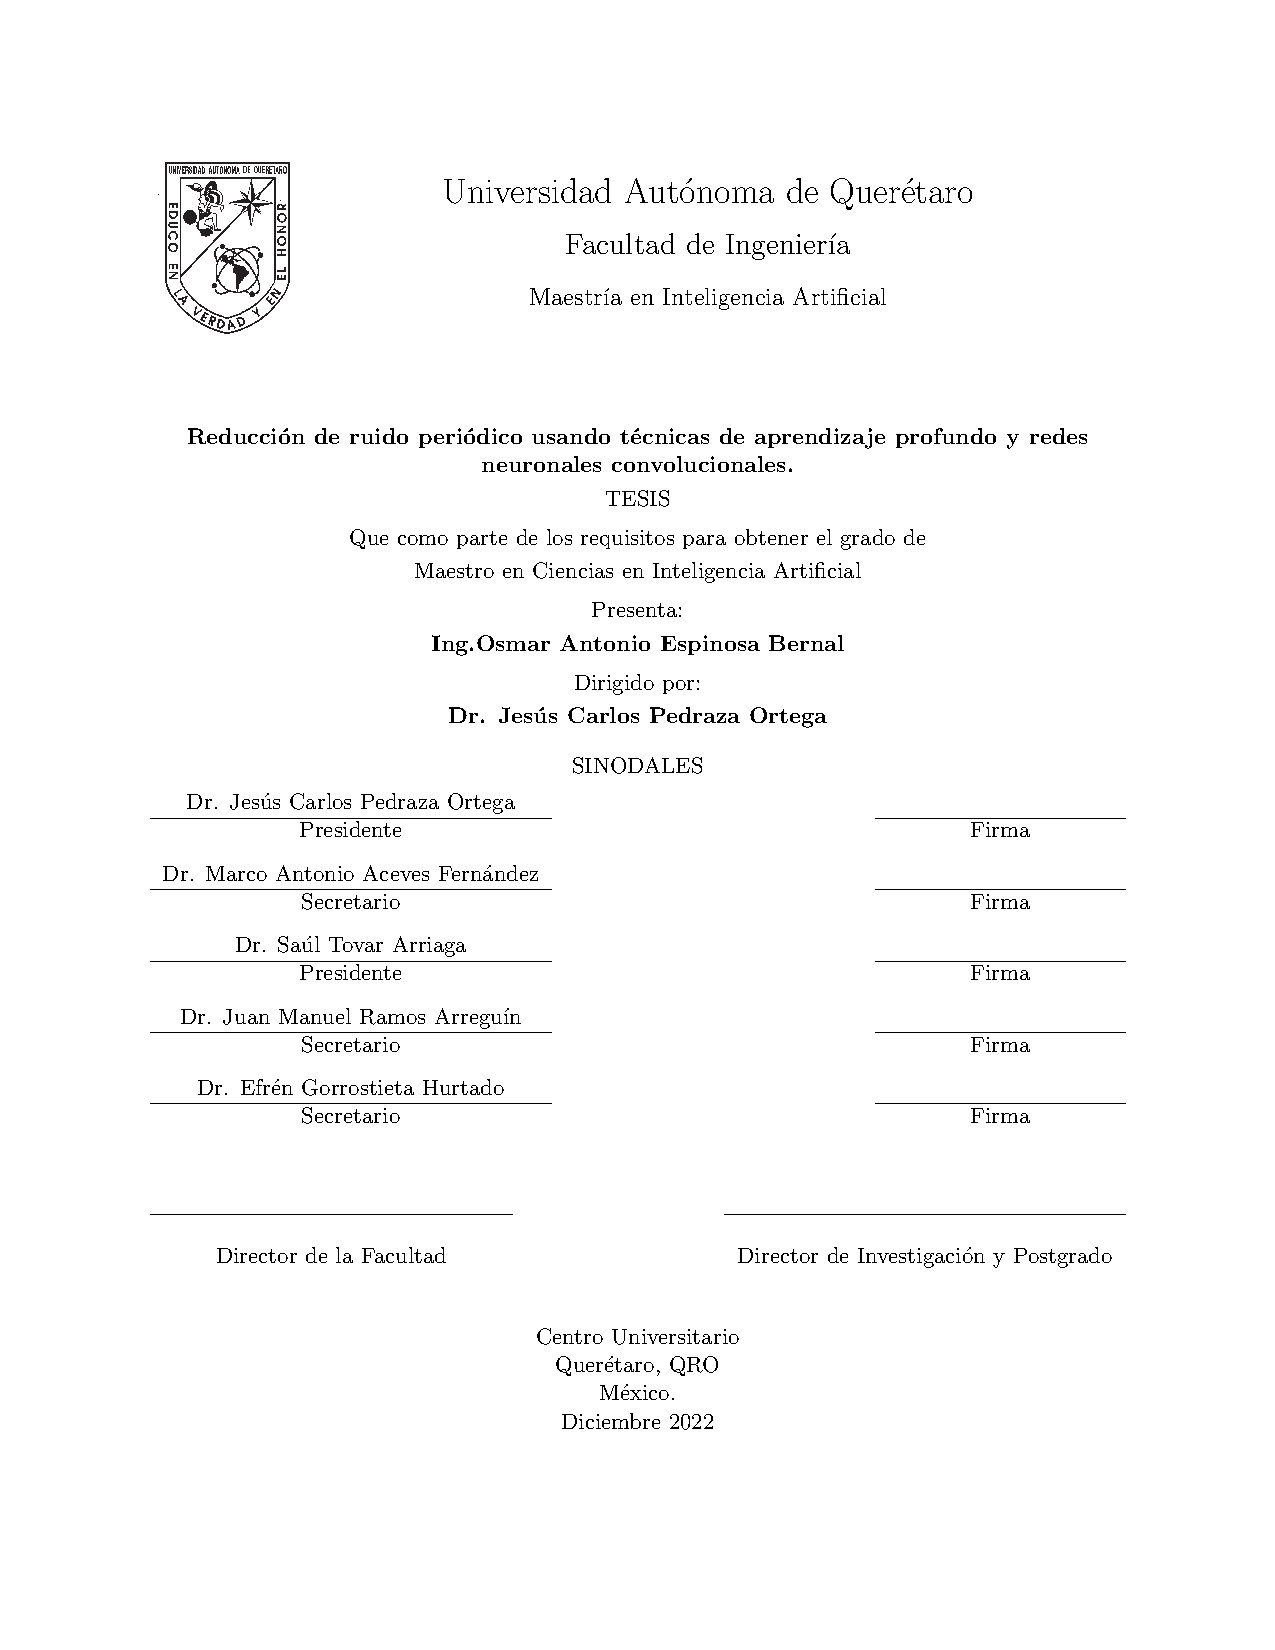
\includepdf[pages=-]{Docus/portadav1.pdf}

%    \begin{titlepage}
%     \centering
%	   \begin{figure}
%            \begin{minipage}{1\linewidth}
%            \centering\centering%\rule{2cm}{2cm}
%%              \caption{Primera figura}
%            \includegraphics[width=0.3\textwidth]{C:/Users/anton/Documents/MCIA/UAQ _MCIA/Sem2_Computo_Evolutivo/Pictures/logos_fi_uaq.png}
%            \end{minipage}
%        \end{figure}
%        
%        {\scshape\LARGE Universidad Autónoma de Querétaro \par}
%	        \vspace{1cm}
%	        
%	    {\scshape\Large División de Investigación y Posgrado \par}
%	        \vspace{1cm}
%	        
%		{\huge\bfseries Tesis\par}
%		    \vspace{1cm}
%		    
%		{\huge\bfseries Reducción de ruido periódico usando técnicas de aprendizaje profundo y redes neuronales convolucionales. \par}	
%		    \vspace{1cm}
%		    
%		{\Large\itshape Función Ackley: Función de optimización\par}
%		    \vspace{1cm}
%		    
%		Director de tesis: Dr. Jesus Carlos Pedraza Ortega \par
%		\vspace{1.2cm}
%		
%		Presenta:\par  \vspace{0.15cm}
%		
%        Ing. Osmar Antonio Espinosa Bernal
%        
%		\vfill
%		% Bottom of the page
%		{\large  06 de diciembre de 2022\par}
%		%{\large 10 de Octubre del 2019\par}
%    \end{titlepage}
%    	%\tableofcontents
%		%\listoffigures
%		%\listoftables
%		\printindex

\tableofcontents
\newpage
\listoffigures
\newpage
\listoftables
\printindex

\newpage
\section{INTRODUCCIÓN}
Sensores y cámaras detectan el mundo en 2 dimensiones y sin profundidad, a diferencia de los humanos que perciben el mundo en 3 dimensiones y con profundidad, detectando de esta manera detalles del mundo que lo rodea.

Sin embargo, técnicas modernas permiten obtener información 3D de objetos mediante sensores y cámaras, consiguiendo de esta manera observar el mundo que lo rodea con cierta precision cercana a la realidad. Una de estas técnicas es la obtención de de información 3D de objetos por medio de imágenes 2D usando perfilometría por cambio de fase (PSP) sobre objetos. Sin embargo, dicha técnica produce patrones de ruido en las imágenes conocido como ruido de Moire que afectan la precisión y reconstrucción final del objeto que se trata de reconstruir y la extracción de información 3D.

En esta tesis se plantea la atenuación con filtro usando técnicas clásicas para reducir la presencia de patrones de ruido de Moire, especificamente ruido cuasi/periódico obtenido durante la extracción y desenvolvimiento de fase(PSP), de imágenes para ser usados en reconstrucciones 3D obtenidos mediante perfilometría por cambio de fase(PSP). La metodología describe detalladamente el procedimiento utilizado para eliminar de manera exitosa el ruido cuasi/periodico. Las imágenes usadas son obtenidas sintéticamente mediante software \textit{Blender} donde fueron capturadas mediante proyección de franjas con un deslizamiento de 120 grados, ademas se obtiene el plano de referencia de usado para recuperar los mapas de fase y las imágenes que contienen la imagen original del objeto sin proyección de franjas y mascara de objeto que se desea reconstruir. Este trabajo propone ademas un filtro basado en una red neuronal convolucional profunda (Deep CNN) para ser usado como pre-procesamiento en la reconstrucción 3D de objetos mediante perfilometría de franjas.

\subsection{Visión por computadora}
El mundo como se nos presenta puede ser percibido en una amplia gama de formas y colores por nuestros ojos. Así podemos darnos cuenta de que le mundo que nos rodea se no presenta en forma tridimensional con tamaño y profundidad variados. Sin embargo las computadoras que reciben esta información mediante sensores de luz como cámaras son incapaces de leer esta información ya que no detectan la profundidad y ni la forma en algunas situaciones de mala iluminación. Con ayuda de sistemas inteligentes de visión los computadores actuales a sido capaces de leer la información de imágenes para obtener información en 3D y ser capaces de reproducirlos tal y como lo hacen los humanos para toma de decisiones. Con la intensión de afrontar este desafió, se han desarrollado técnicas que permiten obtener toda la información disponible a partir de imágenes 2D como entrada.

\subsection{Redes neuronales convolucionales}
Modernas técnicas que permiten extraer la máxima cantidad de información disponible en imágenes 2D con ayuda de Inteligencia Artificial(I.A.) son la redes neuronales convolucionales(CNN). Estas están conformadas por capas de neuronas interconectadas que de acuerdo a la cantidad de capas con que se conforma una red neuronal recibe el nombre de red neuronal de aprendizaje profundo (Deep Learning) que en la practica son mas de dos capas, ya que las capas intermedias estan generalmente ocultas. Las redes neuronales convolucionales son capaces de procesar imágenes para obtener de ellas información mediante obtención mapas de características así como reducción de la resolución de las imágenes de entrada para de esta manera obtener características especificas de dichas imágenes que permitan la clasificación, segmentación o restauración de imágenes.

\subsection{Trabajos relacionados}
Métodos de metrología óptica generan imágenes, como los patrones de franjas haciendo de esta forma esenciales dichas imágenes para reconstrucción 3D. En la mayoría de los métodos interferométricos, una imagen es formada mediante la superposición de las proyecciones de referencia y el objeto a ser medido, con el que se obtiene un patrón de franjas del objeto al ser modulado por una función armónica. Como resultado se obtiene un contraste de zonas iluminadas y zonas oscuras

Las primeras técnicas para obtener mediciones 3D de objetos fue colocando dos rejillas interpuestas que formaban patrones de franjas de Moiré sobre un objeto pequeño. A esta técnica se le conocía como topografía Moiré\cite{Ides:Yata}. % \textbf{Ides:Yata}

Una propuesta diferente de medir objetos 3D fue la perfilometría de la transformada de Fourier, el cual era ajustable y automatizaba las mediciones, lo que le permitía distinguir de esta forma entre una depresión y una elevación de la forma del objeto, no requería asignaciones de orden marginal o determinación de centro marginal y tampoco necesitaba interpolación entre las franjas ya que proporcionaba una distribución de altura de todos los elementos de la imagen sobre la imagen del objeto medido\cite{Take:Muto}. %\textbf{Take:Muto}

Avances tecnológicos permitieron usar proyectores que simulaban las franjas sobre los objetos de manera digital, con lo que se podían manipular mas fácil la proyección de las franjas por la técnica Moiré. De esta manera la franja proyectada podía ser generada de manera digital que permitía la proyección de patrones complejos de franjas. Una  desventaja de los primeros proyectores a color era la proyección de luz solida que son los colores RGB, que cuando se proyectaba el color gris fallaba el sistema. Ademas, los proyectores hacen un ajuste adicional a los patrones que se le envían mediante computador por lo que se distorsiona previamente a la proyección sobre el objeto. Mejoras posteriores permitían la proyección de luz digital. Así, utilizando un proyector de luz infrarroja (Digital-Light Proccesing (DLP)), una cámara infrarroja CMOS de alta velocidad y una cámara a color fue posible la obtención de mediciones de objetos en 3D sin necesidad de proyectar luz visible sobre los objetos, ademas de el color para dar textura al objeto reconstruido. Todo esto en tiempo real e iluminación ambiental\cite{Ou:Li}. % \textbf{Ou:Li}

Otra técnica empleada en la medición de objetos 3D consiste en la aplicación de luz estructurada que es la iluminación activa de la escena con un diseño especial 2D de patrón de intensidad variable espacialmente. Esta iluminación es aplicada sobre una escena por un proyector y una cámara es usada para adquirir la imagen de la escena bajo la iluminación de luz estructurada. El principio de las técnicas de imagen de superficie 3D de luz estructurada es extraer la forma 3D de los objetos basados en la información de la distorsión del patrón proyectado de luz estructurada\cite{Jaso:}\cite{Pedr:Rodr}\cite{Lope:Sala}. %\textbf{Jaso:}\textbf{Pedr:Rodr}\textbf{Lópe:Sala}

Varias técnicas ha sido desarrolladas para extraer información 3D de objetos mediante Perfilometría de Proyección de Franjas también conocido como Perfilometría de Cambio de Fase(PSP) y se especializan en la recolección de datos y análisis que pueden ser aplicados en situaciones donde se requieran mediciones precisas\cite{Ribb:Jaco}. %\textbf{Ribb:Jaco}

El mas reciente avance es la utilización de software que permiten simular la proyección de franjas sobre objetos virtuales y realizar la captura de la imagen para la obtención de información 3D del objeto simulado mediante Perfilometría de cambio de fase.

%%%%%%%%%%%%%%%%%%%% 
\subsection*{Antecedentes de filtros para reducción de ruido en imágenes}  
Las primeras investigaciones para desarrollar filtros en el dominio espacial de las imágenes para reducir el ruido o contaminación lograron eliminarlos de manera limitada, ya que se encontró que estos filtros fallaban debido a que el ruido presente en las imágenes afectaba a toda la imagen, ademas de que, la reducción de ruido no era completa o se perdía información de la imagen \cite{Fehr:Weiss}. %\textbf{Fehr:Weiss} 

La reducción y/o atenuación de ruido o contaminación en imágenes surgió desde que se pudieron conseguir imágenes por medios artificiales. Sin embargo, no fue hasta que se analizaron las fuentes que producían dicha contaminación así como la manera en como se presentan digitalmente que no se comenzó a trabajar en una forma de eliminar ruido presente en imágenes. Con esto se comprobó que existían diferentes tipos de ruido o contaminación en las imágenes. Siendo de particular interés aquellos que aparecían con una periodicidad regular, ya que posteriormente se comprobó que se formaban siguiendo una función definida de tipo sinusoidal.

Una vez que se identifico como se formaba el ruido periódico o cuasi/periódico se se comprobó que llego a la conclusión de que analizando su espectro en el dominio de la frecuencia, se puede identificar que el ruido periódico, siendo este, ruido sinusoidal periódico producido por  diferentes fuentes externas y por el mismo procedimiento de adquisición de información. Sin embargo, el ruido cuasi/periódico es mas difícil de localizar ya que se confunden o mezclan con las características propias de la imagen como se puede observar en las imágenes de la figura \ref{tif313233}.

\begin{figure}[H]
      \begin{center}
        \subfigure[]{
            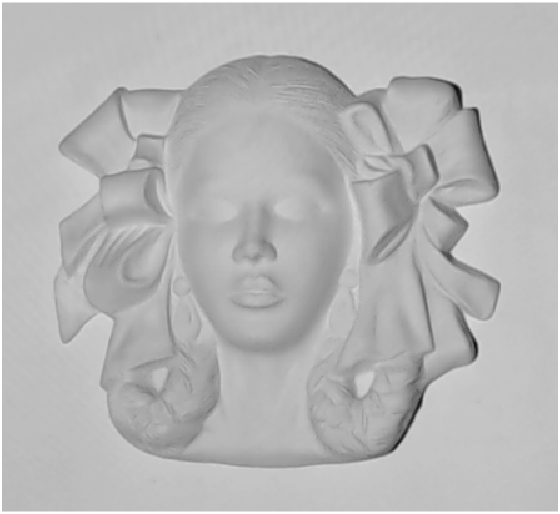
\includegraphics[width=0.3\textwidth]{tifs/tif31.png}
            \label{tif31}}
        \subfigure[]{
            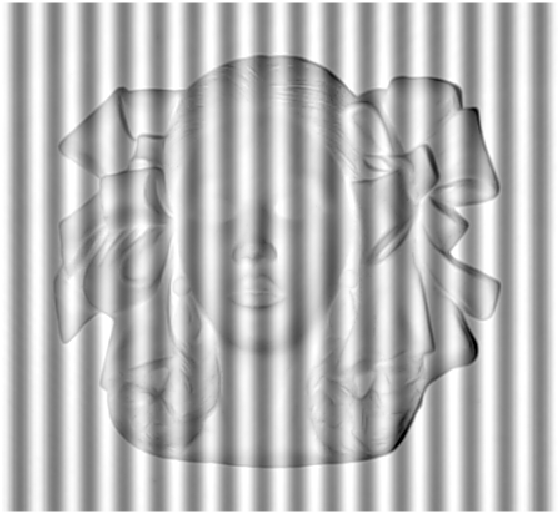
\includegraphics[width=0.3\textwidth]{tifs/tif32.png}
            \label{tif32}}
        \subfigure[]{
            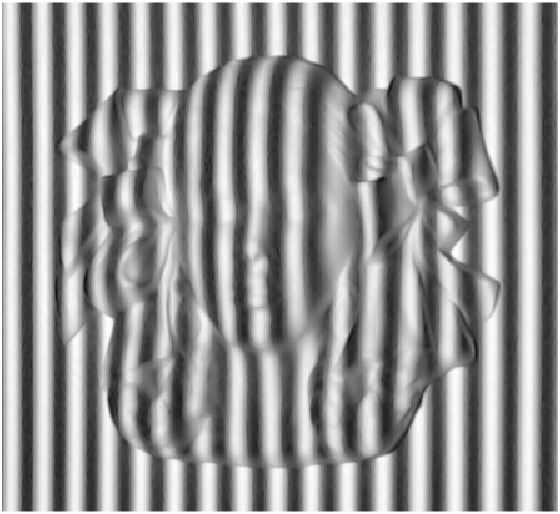
\includegraphics[width=0.3\textwidth]{tifs/tif33.png}
            \label{tif33}}
        \caption{a) Imagen Original, b) Imagen original con ruido periódico y c) imagen original con ruido cuasi/periódico.}
        \label{tif313233}
      \end{center}
    \end{figure}

Sin embargo, aunque se identificaban claramente las regiones que ocasionaban este ruido y se aplicaba un filtro para suprimir o reducir el ruido presente, los costos computacionales eran altos. 

Una vez que se detectaban regiones con ruido en imágenes contaminadas se procedía a su eliminación o atenuación. De esta forma, la aplicación de un filtro de morfología suave (SMF) propuesta por Zhen(Zhen, Zhong, Qi \& Quinghua, 2004)\cite{Zhen:Ming} disminuía el ruido y mejoraba la calidad visual de la imagen, al reemplazar los pixeles de una imagen por el promedio de las salidas de proceso de dilatación y erosión suaves. El filtro de morfología suave optimizado (OSMF) es una variante del filtro SMF que utiliza un enjambre de partículas para optimizar el filtro SMF, sin embargo, las imágenes restauradas contenían un alto grado de distorsión así como de borrosidad por lo que resultaba insuficiente en eliminar o atenuar efectivamente el ruido periódico o cuasi/periódico en imágenes con alto grado de contaminación\cite{Ji:Lu}. %(Ji, Lu 2007) \textbf{Atul:}\textbf{Srin:Cann}\textbf{Lebr:Colo}\textbf{Mila:} 

Investigaciones posteriores trataron la eliminación del ruido presente en imágenes contaminadas mediante su transformación al dominio de la frecuencia de dichas imágenes contaminadas \cite{Atul:}. Al aplicar transformada de Fourier a una imagen contaminada, el ruido periódico o cuasi/periódico aparece como patrones repetitivos. De esta forma las frecuencias del ruido de Moire se concentran como picos de diferente frecuencia perteneciente a un tipo distinto de ruido dependiendo de la función sinusoidal con la que se conforma dicho ruido \cite{Srin:Cann}. Debido a que las frecuencias no deseadas producidas por el ruido periódico o cuasi/periódico se diferencian claramente de las otras frecuencias que componen la imagen, se vuelve relativamente fácil su detección ya que generalmente aparecen con forma de estrella sobre la imagen en el dominio de la frecuencia. De esta forma, filtros basados en el dominio de la frecuencia mejoran la eliminación o atenuación del ruido periódico o cuasi/periódico al reemplazar o suprimir los pixeles corruptos de las regiones que contienen frecuencias corruptas que producen el ruido de Moire\cite{Lebr:Colo}\cite{Mila:}. Diversos filtros basados en el dominio de la frecuencia fueron desarrollados debido al potencial que tenían para reducir y eliminar efectivamente el ruido periódico o cuasi/periódico en imágenes contaminadas. Así, por ejemplo, el filtro de muesca Gaussiano no solo era capaz de filtrar las frecuencias centrales de una región, sino también la de sus vecinos, por lo que aplicando algoritmos de detección de picos de frecuencia, era frecuentemente usado para reducir el ruido de Moire en imágenes corrompidas con este tipo de ruido\cite{Gonz:Rich}. Otros filtros utilizados para el mismo fin como el filtro de muesca Gaussiano por ventanas (Windowed Gaussian Notch Filter)\cite{Aize:Buta} y el filtro de muesca adaptativo optimo (Adaptive Optimum Notch Filter) eran capaces de reducir y atenuar el ruido periódico o cuasi/periódico, sin embargo, su naturaleza no adaptable de detectar regiones con ruido limitaban su rendimiento\cite{Paym:Maso}. %\textbf{Gonz:Rich} \textbf{Aize:Buta} \textbf{Paym:Maso} \textbf{Wei:Wang}

Desde que se descubrió que el patrón de ruido de Moiré también se presentaba en microscopía de rayos x de transmisión de barrido (Scanning Transmision X-ray Microscopy (STXM)), y con ello introduciendo errores significativos en el análisis de imágenes tanto cuantitativos como cualitativos, ademas de la complejidad para evitar el patrón de ruido de Moiré durante la adquisición de imágenes,  Wei, (2011), propuso la introducción de un método de  pos-procesamiento para el filtrado de ruido en imágenes STXM. El método incluye una detección semiautomática de picos presentes en la amplitud de espectro de Fourier\cite{Wei:Wang}. Una vez localizados las regiones afectadas por ruido de Moire, Alvarado (Alvarado, 2020) propone un filtro de cruz, que suprime las frecuencias de ruido localizadas a lo largo de los ejes vertical y horizontal de las imágenes en el dominio de la frecuencia, consiguiendo con ello atenuar exitosamente el ruido cuasi/periódico en imágenes obtenidas mediante proyección de franjas\cite{Alva:Orte}. %\textbf{Alva:Orte}

Filtros con umbral adaptativo basados en el dominio de la frecuencia como el filtro ATBF (Adaptative Threshold Based Filter) propuesto por Varghese(Varghese, 2016),  es efectivo para reducir el ruido periódico mediante la determinación adaptativa de una función de umbral para la identificación de áreas con un pico de ruido en el dominio de la frecuencia de una imagen. Después las frecuencias corruptas son difuminados por un filtro de mínimos para una restauración en el dominio de la frecuencia de las imágenes. La imagen restaurada en el dominio de la frecuencia se le aplica la transformada de Fourier inversa y operaciones de cambio para reconstruir la imagen final al dominio espacial\cite{Varghese:}. Sin embargo, no es completamente efectivo en imágenes que contienen ruido cuasi/periódico dada la naturaleza de dicho ruido. %\textbf{Varghese:}\textbf{Gonz:Rich} 

Filtro de suavizado espaciales se han usado para difuminar imágenes logrando de esta forma reducir o atenuar el ruido periódico o cuasi/periódico presente en imágenes digitales. De esta forma, aplicando filtros lineales, se puede eliminar el ruido en imágenes contaminadas. Al aplicar un filtro de suavizado espacial, dicho filtro consiste en simplemente realizar un promedio de pixeles vecinos y reemplazar un pixel con dicho valor\cite{Gonz:Rich}. Otras técnicas aplicadas al dominio espacial para atenuar el ruido periódico o cuasi/periódico de imágenes contaminadas incluyen algoritmos que remueven la textura de imágenes contaminadas ya que contiene componentes de ruido periódico o cuasi/periódico de alta frecuencia\cite{Kara:Erde}\cite{Ono:Miya}\cite{Ok:Youn}. %\textbf{Kara:Erde} \textbf{Ono:Miya} \textbf{Ok:Youn} \textbf{Kriz:Suts} \textbf{Simo:Ziss}  \textbf{Szeg:Liu} \textbf{Dong:Loy} \textbf{Ghar:Chaur}\textbf{Ghar:Chaur} \textbf{Zhan:Zuo}

Recientes técnicas hacen uso de redes neuronales convolucionales después de demostrar que eran capaces de clasificar\cite{Kriz:Suts} y reconocer imágenes\cite{Simo:Ziss}\cite{Szeg:Liu}, ademas de que han demostrado su potencial en áreas de visión por computadora de bajo nivel y tareas de procesamiento de imagen. Tareas como imágenes con super-resolución\cite{Dong:Loy}, reconstrucción de imágenes mediante muestras cromáticas incompletas\cite{Ghar:Chaur}, eliminación de ruido\cite{Ghar:Chaur} y restauración de imágenes \cite{Zhan:Zuo}, son aplicaciones en constante evolución. Usando un red neuronal convolucional profunda (DnCNN), Zhang, 2017, consigue remover el ruido blanco de imágenes contaminadas en diferentes niveles utilizando estrategias de eliminación de ruido de aprendizaje residual limpiando imágenes dentro de las capas ocultas del modelo DnCNN\cite{Zhan:Zuo1}. Sun(Sun, Yu, \& Wang, 2018)\cite{Sun:Yu} propone una red neuronal convolucional profunda para eliminar el ruido de Moire de imágenes capturadas con cámaras fotográficas de celulares. %\textbf{Zhan:Zuo1} 

Técnicas de perfilometría de superficie y pre-procesamiento de imágenes con CNN para eliminación de ruido están en constante desarrollo debido a la gran demanda que se tiene en el campo científico por su gran exactitud y rapidez que se consiguen, aproximándose al objeto real. Sin embargo, aun existe el desafió de conseguir superficies complejas como el rostro humano entre otros.


\subsection{Estado del arte}
En la tabla 1 se muestran los antecedentes recopilados mas relevantes que se han realizado sobre técnicas para reducir el ruido periódico en imágenes.

\begin{table}[H]
\centering
%\resizebox{12cm}{5cm} {
\caption{Tabla de autores con los antecedentes mas relevantes.}
\begin{turn}{90}
\begin{tabular}{ p{3.5cm} p{3.5cm} p{3.5cm} p{6cm}}
\hline
Autor(es)& Técnica & Uso de Técnica & Aportación \\
\hline \hline
Wei, Z., (2012) & Filtro Gaussiano de la mediana. & Remover ruido periódico & Detección y corrección de distorsiones en el espectro en imágenes  causados por ruido periódico. \\
\hline
Varghese, J., (2016) & Filtro de dominio de frecuencia basado en umbral adaptativo. & Reducción de ruido periódico presente en imágenes & Identificación de frecuencias con ruido en dominio de la frecuencia en imágenes y restauración de dichas frecuencias corruptas.   \\
\hline
Van der Jeught S, (2016) & Perfilometría. & Estado del arte & Dar a conocer los métodos más comúnmente utilizados para la reconstrucción y la medición de superficies 3D.\\
\hline
Sun, Y., (2018) & Uso de redes neuronales convolucionales multiresolución. & Remoción de patrones de Moiré en imágenes & Reducción de patrones de Moiré mas significativas comparados con otros métodos. \\
\hline
Ji, Z., (2004) & Filtro de morfología suave. & Reducir el ruido periódico presente en el procesamiento de imágenes & Diseño e implementación en computación mas eficiente que otros métodos convencionales en el dominio de la frecuencia. \\
\hline
Nah, S., (2017) & Aprendizaje residual y normalización por lotes de DeepCNN. & Eliminación de ruido en imágenes & Alta efectividad para eliminar ruido e implementación eficiente haciendo uso de GPU (Graphics Processing Unit). \\
\hline
Alvarado Escoto L. A. (2020) & Filtro bilateral & Procesamiento de imágenes para reconstrucción de objetos 3D & Reconstrucción de objetos mas suaves y mejor estimación de alturas de los objetos reconstruidos. \\

\hline
\end{tabular}%}
%\caption{Tabla de autores con los antecedentes mas relevantes.}
\label{tabla:autores}
\end{turn}
\end{table}

\subsection{Definición del problema}
Actualmente la generación de un objeto 3D por computadora a partir de lectura de objetos utilizando técnicas como perfilometría a tomado relevancia debido a las muchas aplicaciones posibles en diversas áreas lo que ha abierto un nuevo campo de investigaciones para este fin. Sin embargo la reconstrucción de objetos presenta aun problemas debido al ruido cuasi/periódico producido durante el procedimiento de adquisición de las imágenes. Este ruido es adquirido por el desplazamiento de franjas sobre el objeto que se desea reconstruir ya que genera deformaciones sobre el objeto cuando encuentra zonas con geometría compleja o con sombras, entre otros.

Además, la proyección de múltiples patrones de franjas también genera interferencia, debido a que cuando se procesan en conjunto, se traslapan entre ellas produciendo el ruido de Moire. Otro problema se produce cuando se intenta reconstruir un objeto tridimensional en movimiento, ya que la proyección de franjas presenta una mayor interferencia entre ellas, produciendo un mayor traslape entre las proyecciones y en consecuencia, mayor ruido cuasi/periódico en la reconstrucción del objeto tridimensional.    

La obtención de medidas cercanas a los reales es un problema aun presente en la generación de objetos 3D por computadora debido a que son fuertemente afectados por el ruido presente en la imágenes utilizadas para tal fin lo que genera un objeto final reconstruido inexacto o poco confiable impidiendo su uso en aplicaciones donde la precisión es un factor importante. 

Las investigaciones actuales aunque han mejorado siguen presentando este problema en la reconstrucción de objetos 3D por lo que los sistemas para eliminar el ruido periódico de las imágenes antes del proceso de generación del objeto 3D usando redes neuronales convolucionales (CNN) podría reducir el ruido sobre las imágenes antes de la reconstrucción del objeto 3D consiguiendo de esta manera una mayor precisión en la reconstrucción del objeto 3D por computadora.

\subsection{Justificación}
Actualmente, la obtención y reconstrucción de imágenes tridimensionales esta en pleno desarrollo con los avances tecnológicos y metodológicos que se han alcanzado. Sin embargo, la fase de reconstrucción final del objeto tridimensional sigue presentando desafíos aun por resolver como el ruido periódico y cuasi/periódico, ademas de los patrones de Moire producidos por el movimiento de los objetos, y por interferencia entre los píxeles de una pantalla y los píxeles del sensor de la cámara, esto es por que el objeto final generado por computadora, presenta irregularidades que no son deseados, como imprecisiones cuando se  realizan mediciones debido a que no se genera completamente el objeto por el ruido presente en las imágenes que se toman como modelo.

Los avances en el desarrollo de redes neuronales convolucionales para restauración de imágenes permiten reducir el ruido presente en imágenes antes de generar el objeto final, lo que supondría un avance en este campo ya que se traduciría en una mejor precisión al obtener el objeto final reconstruido, además debido a que hacen uso de la Unidad de Procesamiento Gráfico (GPU) aumentaría de la velocidad de procesamiento lo que también provocaría una disminución en los tiempos de procesamiento de imágenes reduciendo también costos, haciendo posible su implementación en áreas de aplicación en los que actualmente se demandan una mayor precisión de objetos tridimensionales reconstruidos a partir de imágenes y en tiempo real.

La aplicación de objetos reconstruidos de manera tridimensional obtenidos con precisión podría tener aplicaciones en diferentes áreas como medicina, donde seria posible crear prótesis, piezas dentales, entre otros. Otra aplicación de interés tiene que ver con la generación de entornos virtuales ya que facilitaría la generación de objetos de formas irregulares, entre otros. 

\subsection{Hipótesis}
Un filtro basado en aprendizaje profundo reduce el ruido periódico presente en imágenes adquiridas por perfilometría permitiendo una reconstrucción de objetos 3D por computadora mas aproximadas, comparables al estado del arte.

\subsection{Objetivos}
\subsubsection{Objetivo general}
Desarrollar e implementar un filtro de reducción de ruido periódico basado en aprendizaje profundo para la reconstrucción 3D de objetos con el objetivo de mejorar la exactitud.

\subsubsection{Objetivos específicos}
\begin{itemize}
\item Realizar un análisis del tipo de ruido periódico presente en imágenes obtenidas por perfilometría para conocer sus características.

\item Proponer un filtro basado en una arquitectura CNN para reducir el ruido periódico de las imágenes antes de su reconstrucción.

\item Realizar pruebas aplicando el filtro desarrollado a imágenes con ruido periódico para medir los resultados de la implementación y compararlo con otras metodologías del estado del arte.

\end{itemize}

\subsubsection{Alcances}

\begin{itemize}
\item Desarrollar un algoritmo que reduzca ruido de Moire presente en imágenes para su uso en reconstrucción 3D de objetos.

\item Crear base de datos con imágenes que se usaran para experimentación.

\item Proponer una arquitectura de Red Neuronal Convolucional que reduzca ruido de Moire presente en imágenes.

\item Realizar las pruebas y experimentos requeridos para concluir con el proyecto.
\end{itemize}

\subsubsection{Limitaciones}
\begin{itemize}
\item Tiempo limitado para la consecución de imágenes para entrenamiento de red neuronal convolucional.

\item Falta de equipo adecuado para entrenamiento de red neuronal convolucional(CNN)
\end{itemize}

%\subsection{Organización de la tesis}


\section{REVISIÓN DE LITERATURA}
La reconstrucción 3D de objetos es una tarea complicada que se realiza con el fin de obtener objetos digitales que pueden ser usados en muchas aplicaciones. Los modelos 3D no deben ser en muchos casos solo visualmente similares al objeto real, sino también deberían ser precisos desde un punto de vista geométrico. Algunas técnicas de escaneo permiten reconstruir objetos a partir de escaneos de objetos de manera digital. Para reconstrucción de objetos 3D a partir de imágenes existen diferentes técnicas, las cuales pueden ser clasificadas en 2 grupos: técnicas por contacto y técnicas sin contacto\cite{Rocc:Cign}. %\textbf{Rocc:Cign} 

La figura \ref{tif34} muestra las diferentes técnicas existentes de contacto y no contacto para reconstrucción de objetos 3D.

\begin{figure}[H]
	\centering
    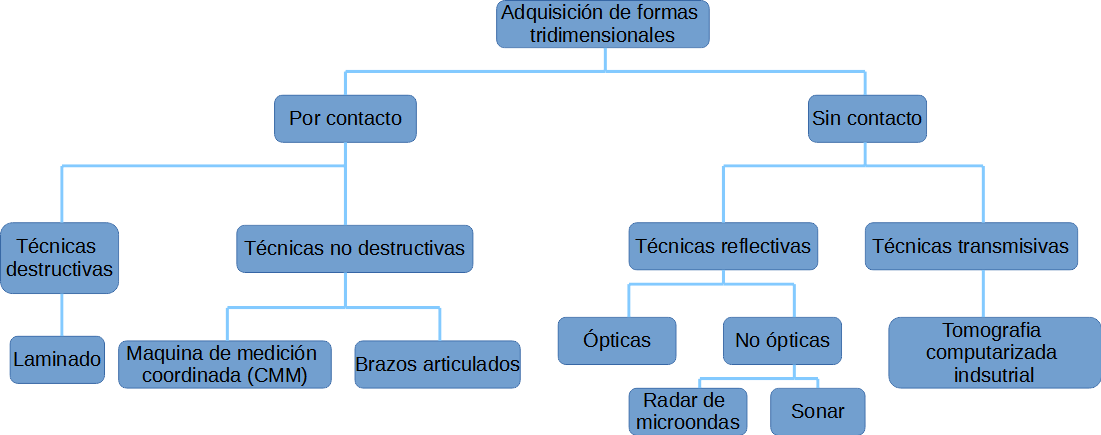
\includegraphics[width=1\textwidth]{tifs/tif34.png}
    \caption{Taxonomía de las técnicas de adquisición 3D\cite{Rocc:Cign}.}
    \label{tif34}
\end{figure}

Las técnicas por contacto tienen el inconveniente de que pueden ser destructivas y estar en contacto directo con el objeto, lo que puede ocasionar daño al objeto. Las técnicas sin contacto por otro lado solo toman escaneos del objeto por lo que el daño invasivo con el objeto es mínimo. Estos se dividen a su vez en reflectivas y transmisivas. Las técnicas reflectivas a su vez se dividen en ópticas y no ópticas. La figura \ref{tif35} muestra la clasificación de técnicas ópticas. 

\begin{figure}[H]
	\centering
    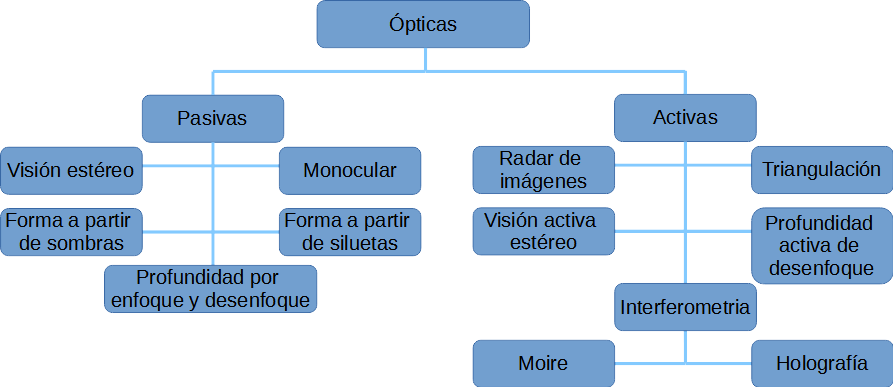
\includegraphics[width=1\textwidth]{tifs/tif35.png}
    \caption{Clasificación de las técnicas de adquisición óptica\cite{Rocc:Cign}.}
    \label{tif35}
\end{figure}

Diferentes técnicas ópticas han sido implementados para reconstruir objetos en 3D de manera precisa y similar al objeto real mediante adquisición de la información del objeto por medios ópticos. Así se han desarrollado sistemas de visión estéreo, luz estructurada y tiempo de vuelo, sin embargo la técnica de luz estructurada a sobresalido por sobre las demás técnicas debido a su simplicidad y velocidad de procesamiento\cite{Ou:Li}. Extracción de información 3D mediante técnicas de luz estructurada se basa en las técnicas de codificación de luz proyectada y proyección de patrón de franjas sinusoidal, en el cual la profundidad del objeto es extraído mediante la deformación de un patrón de franjas proyectado sobre un objeto\cite{Yosh:}. %\textbf{Ou:Li}\textbf{Yosh:} 

\subsection{Principio de perfilometría de proyección de franjas y desenvolvimiento de fase}
La idea principal de perfilometría mediante proyección de franjas es obtener un mapa de alturas de un objeto dado como un mapa de patrón de franjas deformado. Al mismo tiempo se obtiene el contorno del objeto permitiendo de esta forma visualizar características físicas del objeto\cite{Yosh:}. %\textbf{Yosh:} 

Como se observa en la figura \ref{tif36}, un sistema básico de perfilometría por proyección de franjas consiste en una cámara, un proyector y el patrón definido de franjas que se proyectara sobre un objeto, el objeto y el mapa de referencia de dicho objeto que es simplemente la proyección de franjas sin el objeto.

\begin{figure}[H]
	\centering
    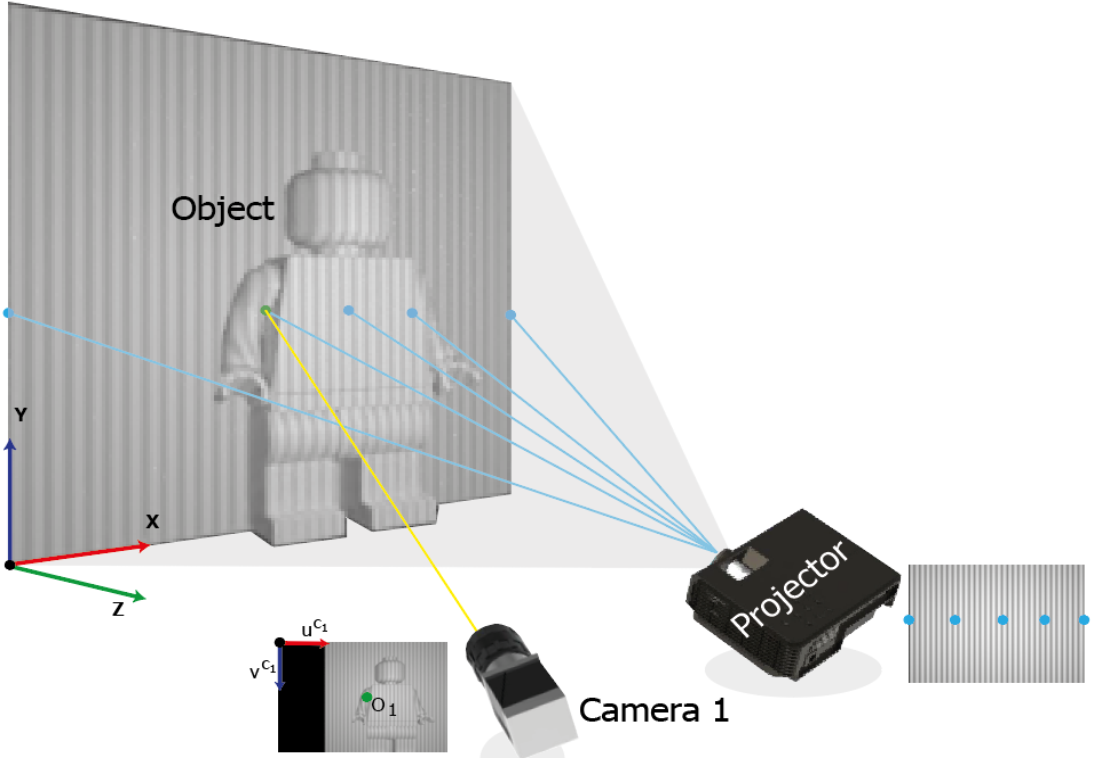
\includegraphics[width=0.6\textwidth]{tifs/tif36.png}
    \caption{Sistema básico de perfilometría de proyección de franjas.}
    \label{tif36}
\end{figure}

Diferentes patrones de pueden ser usados para la proyección de franjas, sin embargo, los mas usados son barras verticales que pueden tener una disposición diferente. La figura \ref{tif373839} muestra diferentes vistas de la proyección de franjas representadas por barras.

\begin{figure}[H]
      \begin{center}
        \subfigure[]{
            
\includegraphics[width=0.3\textwidth]{tifs/tif39.png}
            \label{tif39}}
        \subfigure[]{
            
\includegraphics[width=0.3\textwidth]{tifs/tif38.png}
            \label{tif38}}
        \subfigure[]{
            
\includegraphics[width=0.3\textwidth]{tifs/tif37.png}
            \label{tif37}}
        \caption{Diferentes patrones de barras usados en perfilometría de proyección franjas.}
        \label{tif373839}
      \end{center}
\end{figure}


El algoritmo de cambio de fase de N-pasos (N-Step) es un método conocido por su insensibilidad a la luz ambiental y reflectividad de la superficie\cite{Tao:Chen}, donde una serie patrones con deslizamiento de fase son proyectados con un cambio de fase obteniendo con ello un conjunto de imágenes que depende del numero de pasos siendo estos de 3, 4, 8 o 12 pasos entre otros (N-Step). Los patrones de franjas pueden ser expresados teóricamente en una imagen como la ecuación \ref{fringe-pattern}: %\textbf{Tao:Chen}

\begin{eqnarray}
\label{fringe-pattern}
I(x,y)=a(x,y)+b(x,y)cos(\phi (x,y))
\end{eqnarray}

Existen varias maneras de extraer la información 3D de un objeto basados en el análisis de proyección de franjas tales como deslizamiento de fase y transformada de Fourier. Entre las técnicas mas comunes usados para la extracción de información 3D se encuentran: Perfilometría transformada wavelet (Wavelet Transform Profilometry (WFP)), (Spatial Filtered Profilometry (SFP)) y Perfilometría por Transformada de Fourier (Fourier Transform Profilometry (FTP)) siendo este ultimo la mas comúnmente usada cuando se tiene una única imagen de entrada. En FTP, un patrón sinusoidal de Ronchi se proyecta sobre la superficie de un objeto. Entonces la profundidad del objeto es codificado mediante un patrón de franjas deformado que puede ser decodificado usando la transformada de Fourier filtrando en el dominio espacial y usando la transformada inversa de Fourier, teniendo como ventaja, evitar la interpolación de franjas, ya que se obtiene una distribución de altura en cada pixel en todo el campo de calculo\cite{Su:Chen}. %\textbf{Su:Chen}

%Una vez ajustado el sistema de perfilometria por proyección de franjas emulado, 
Los patrones de deslizamiento de fase proyectados para 3 pasos (3-Step) quedan como se muestra en las ecuaciones \ref{three-stepv1}, \ref{three-stepv2} y \ref{three-stepv3}.

\begin{eqnarray}
\label{three-stepv1}
I_{L0}=A_L+B_Lcos\left ( \phi _L \right )
\end{eqnarray}

\begin{eqnarray}
\label{three-stepv2}
I_{L0}=A_L+B_Lcos\left ( \phi _L +2\pi /3\right )
\end{eqnarray}

\begin{eqnarray}
\label{three-stepv3}
I_{L0}=A_L+B_Lcos\left ( \phi _L +4\pi /3\right )
\end{eqnarray}


Con el algoritmo de deslizamiento de fase, la fase envuelta $\phi$ para N-Pasos (N-Step)\cite{Schr:Brun} puede ser obtenido mediante la ecuación \ref{wrapped-phase} por el método de mínimos cuadrados. 

\begin{eqnarray}
\label{wrapped-phase}
\phi_L=artan\frac{\sum_{n=0}^{N-1}I_{cn}sin\left ( 2\pi n/N \right )}{\sum_{n=0}^{N-1}I_{cn}cos\left ( 2\pi n/N \right )} 
\end{eqnarray}

Entonces la fase envuelta $\phi$ usando el método de 3 pasos (3-Step) puede ser calculada con la ecuación \ref{wrapped-phase-3-step}.

\begin{eqnarray}
\label{wrapped-phase-3-step}
\phi_L=artan\frac{\sqrt{3}\left ( I_{L1}- I_{L2}\right )}{2\left (I_{L0}-I_{L1}-I_{L2} \right )} 
\end{eqnarray}

Dada la naturaleza de la función arctan, los valores extraídos oscilaran entre $[-\pi,+\pi]$, es posible que la fase real se encuentre en intervalos mas grandes que $2\pi$ dando como resultado una fase recuperada con discontinuidades artificiales.

La fase absoluta $\Phi _L$ y la fase envuelta $\phi _L$ satisfacen la siguiente relación:

\begin{eqnarray}
\label{abs-wrapped-phase}
\Phi _L= \phi _L +2k\pi
\end{eqnarray}

donde $k$ es el orden de periodo, $k \in [0,N_L-1]$ y $N_L$ denota el numero de franjas proyectadas en el plano marginal del sistema. 

El mapa de fase obtenido contiene saltos de fase en pixeles adyacentes desde $+\pi$ a $-\pi$ y viceversa, por lo tanto es necesario conectar los saltos de fase para obtener una distribución física final. La fase envuelta puede expresarse como la ecuación \ref{wrapped-phase2} donde $x(n)$ es la fase continua original, $W[\;\;]$ en el operador de la fase y $x_w(n)$ es la fase envuelta.

\begin{eqnarray}
\label{wrapped-phase2}
x_w(n)= W[x(n)]
\end{eqnarray}

El desenvolvimiento de fase  es un proceso que determina la integral múltiple desconocida de $\pi$ que sera sumado a cada pixel de la fase envuelta previamente adquirida para hacer la señal de la fase continua en el dominio de la frecuencia. Removiendo todas las discontinuidades artificiales de $2\pi$ se obtiene la fase original después de aplicar la función de arctan, proceso que es realizado mediante la comparación de los pixeles vecinos de un pixel dado, y sumando o restando $2\pi$ para obtener la fase relativa entre ambos pixeles en el rango de $-\pi$ a $+\pi$. Sin embargo, el proceso puede ser difícil debido a la presencia de sombras, modulaciones de franjas bajas, discontinuidades de las franjas, ruido en la imágenes entre otros\cite{Gort:Rast}. %\textbf{Gort:Rast}

\subsection{Patrón de Moire}

Cuando 2 patrones similares repetitivos de lineas, círculos o puntos se sobreponen una sobre la otra sin alineación, aparece un nuevo patrón dinámico llamado ruido de Moire. El ruido de Moire puede modificar la forma y frecuencia de sus elementos cuando se mueven relativamente uno contra el otro degradando de esta forma la calidad visual de una imagen como se puede observar en las imágenes de la figura \ref{tif313233}\cite{Sun:Yu}. %\textbf{Sun:Yu}

Se puede observar en la figura \ref{tif32} el patrón periódico que presenta la imagen y como se degrada la calidad visual de la misma, mientras que la figura \ref{tif33} se aprecia que el patrón es cuasi-periódico ya que las franjas que muestra la imagen se adapta al objeto mismo, teniendo como resultado una mayor degradación visual de la imagen.

Durante años se han desarrollado técnicas que reduzcan este patrón de Moire debido a la demanda de imágenes limpias, claras y de alta resolución. Varias de esas técnicas operan sobre el dominio de la frecuencia de las imágenes analizando su espectro de amplitud y detectando picos de alta frecuencia. Otra técnica es la descomposición de matriz dispersa para el tratamiento de patrones Moiré\cite{Alva:Orte}. Otras aproximaciones mas recientes hacen uso de redes neuronales convolucionales(CNN). %\textbf{Alva:Orte}\textbf{Wei:Wang}

En PSP, los patrones de Moire aparecen debido a la naturaleza del patrón de franjas usado y puede ser difícil controlar su aparición durante la adquisición de las imágenes. Por lo tanto un pos-procesamiento es realizado para remover o reducir el patrón de Moire siendo procesado normalmente sobre el dominio de la frecuencia de la imagen mediante la corrección de los componentes alterados por el ruido en el espectro de amplitud consiguiendo de esta manera objetos reconstruidas en 3D mas suaves, precisas y aproximadas al objeto real\cite{Wei:Wang}. 

\section{METODOLOGÍA}
\subsection{Perfilometría por cambio de fase}
El método por cambio de fase para obtener información de un objeto 3D es uno de los métodos ópticos que consigue tener menos error respecto del objeto original cuando se compara con otras técnicas. Este método consiste en la proyección de de franjas sobre un objeto usando un proyector y una cámara para obtener imágenes en diferentes posiciones para capturar la modulación o distorsión de dichas franjas con la forma del objeto repitiendo el proceso con un desplazamiento de las franjas proyectadas sobre el objeto.

\subsubsection{Algoritmo de 3 pasos (three-step)}
Uno de los algoritmos mas usados en la perfilometría de cambio de fase es el método de 3 pasos (three-step). El método proyecta sobre el objeto 3 patrones de franjas. Estos patrones son descritas mediante las ecuaciones \ref{three-step1}, \ref{three-step2} y \ref{three-step3}.

\begin{eqnarray}
\label{three-step1}
I_1=I'\left ( x,y \right )+I''\left ( x,y \right )Cos(\phi \left ( x,y \right ))
\end{eqnarray}

\begin{eqnarray}
\label{three-step2}
I_2=I'\left ( x,y \right )+I''\left ( x,y \right )Cos(\phi \left ( x,y \right )+\alpha)
\end{eqnarray}

\begin{eqnarray}
\label{three-step3}
I_3=I'\left ( x,y \right )+I''\left ( x,y \right )Cos(\phi \left ( x,y \right )+ 2\alpha)
\end{eqnarray}

donde $I'\left ( x,y \right )$ es la intensidad, $I''\left ( x,y \right )$ es la intensidad de modulación, $\phi \left ( x,y \right )$ es la fase verdadera y $\alpha$  es el desfase igual a $2\pi/3$ \cite{Kato:}\cite{Schr:}\cite{ Garc:}.

\subsection{Adquisición de imágenes}
Para obtener las imágenes con la proyección de franjas se desarrolla un entorno de emulación desarrollado en \textit{Blender}, que es un software de uso libre para cualquier propósito ya se comercial o educativo. Para la extracción y generación de figuras 3D se utilizaron figuras desarrolladas por profesionales en el campo y que pueden ser obtenidos de paginas como \textit{TurboSquid}. \textit{TurboSquid} es usado por profesionales y desarrolladores de todo el mundo y fue creado con la intención de ahorrar tiempo en el desarrollo de modelos 3D grandes y complejos permitiendo aprovechar el tiempo en otras áreas de desarrollo.

El sistema utilizado en software \textit{Blender} consiste en elementos como cámaras, objetos 3D y luces. Con las luces se emula las franjas que se proyectan sobre los objetos simulando el sistema de perfilometría por proyección de franjas que consiste en un proyector que es representado por una lampara con configuración mostrada mas adelante, una cámara con una longitud de 28 mm con una lente de tipo "Perspectiva" en Configuración de Cámara como se muestra en la figura \ref{tif1} donde $P$ es el centro de la proyección del proyector, $C1$ es el centro de imágenes de la cámara, $D$ es un punto arbitrario del objeto de prueba y el área efectiva de proyección de 15.4 mm es representado por$l_0$. La distancia $d$ entre la cámara y el proyector es de 3 mm y el plano de referencia es colocado frente al proyector a aproximadamente 15 mm representado por $l$. El entorno de emulación es realizando en \textit{Blender} version 2.95.5.\cite{Mart:Suar}. 

\begin{figure}[H]
	\centering
    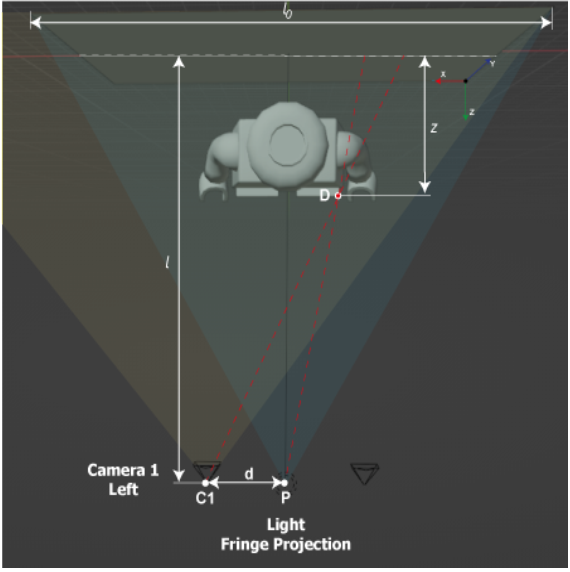
\includegraphics[width=0.5\textwidth]{tifs/tif1.png}
    \caption{Trayectoria óptica de la perfilometría de medición de fase en el entorno emulado.}
    \label{tif1}
\end{figure}

El árbol de nodos generados crea un plano de proyección como se muestra en la figura \ref{tif2} seguido de un bloque llamado CLIP donde se generan los limites de la proyección de las lamparas a un área especifica. Debajo de cada bloque anterior tenemos un bloque llamado SINE que genera la proyección de franjas ademas de ser el bloque donde se puede manipular el cambio de fase de acuerdo al numero de pasos que se implementara en este caso de 3 pasos(3-Step).

\begin{figure}[H]
	\centering
    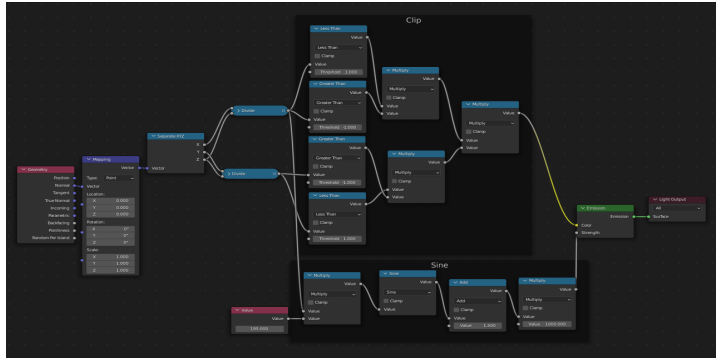
\includegraphics[width=0.8\textwidth]{tifs/tif2.png}
    \caption{El árbol principal de nodos de composición de este sistema \textit{Blender}.}
    \label{tif2}
\end{figure}

Los objetos virtuales que se usaron pueden ser encontrados en el sitio \textit{TurboSquid}, pero también pueden ser encontrados en base de datos  \cite{Wang:Wang} tales como ModelNet, ShapeNet, ABC, Thingi10K, etc., donde una variada colección de objetos desde simples a complejos pueden usarse para adquirir las imágenes con proyección de franjas sobre los objetos, como se muestra en los modelos de la figura \ref{tif3}.  %\textbf{Wang:Wang} 

\begin{figure}[H]
	\centering
    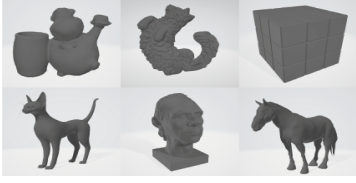
\includegraphics[width=0.8\textwidth]{tifs/tif3.png}
    \caption{Modelos del sitio \textit{TurboSquid}.}
    \label{tif3}
\end{figure}

Con el sistema de emulación del proyección de franjas se obtienen imágenes con una resolución de 640 pixeles de ancho por 480 pixeles de alto y la generación de cada imagen renderizada toma un promedio de 1 segundo que puede variar debido a la complejidad del objeto. Las imágenes obtenidas consisten en un conjunto de 3 imágenes con la proyección de franjas con deslizamiento de fase de $2\pi/3$ sobre el objeto y 3 con la proyección de imágenes si objeto para obtener la referencia, una(1) imagen de GroundTruth y una(1) imagen mascara del objeto para obtener una región de interés sobre el objeto. De esta manera se obtienen 8 imágenes por cada escena que se monta con el sistema.

\begin{figure}[H]
      \begin{center}
        \subfigure[]{
            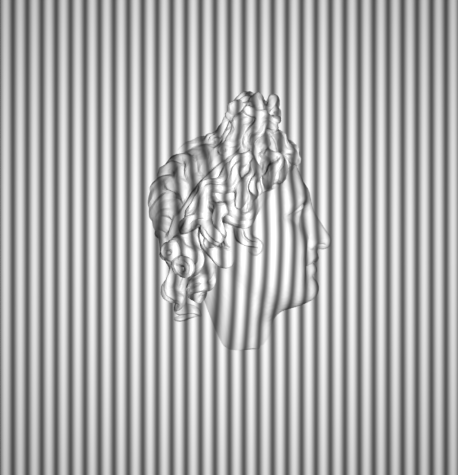
\includegraphics[width=0.3\textwidth]{tifs/tif4.png}
            \label{tif4}}
        \subfigure[]{
            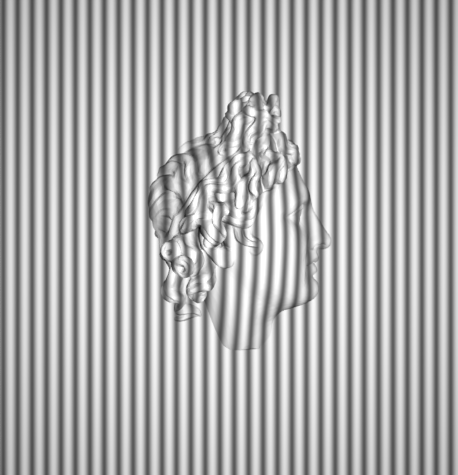
\includegraphics[width=0.3\textwidth]{tifs/tif5.png}
            \label{tif5}}
        \subfigure[]{
            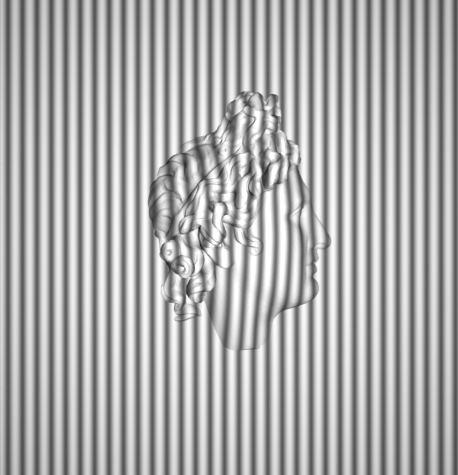
\includegraphics[width=0.3\textwidth]{tifs/tif6.png}
            \label{tif6}}
        \subfigure[]{
            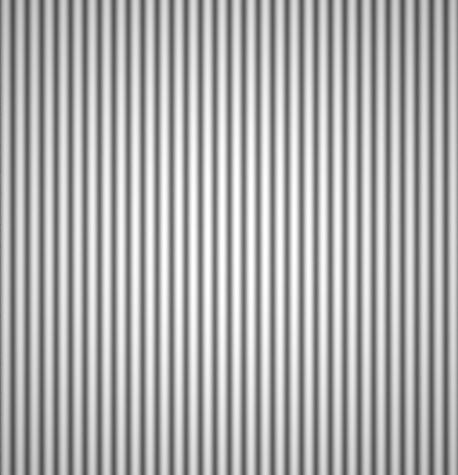
\includegraphics[width=0.3\textwidth]{tifs/tif7.png}
            \label{tif7}}
        \subfigure[]{
            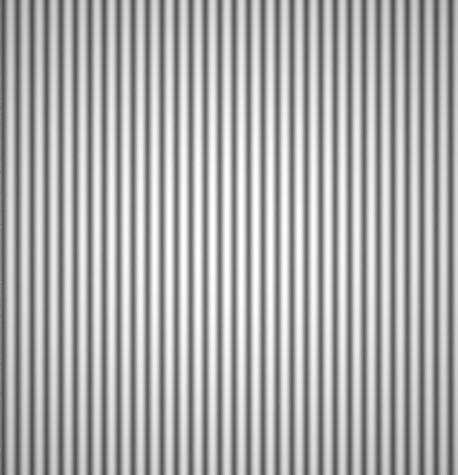
\includegraphics[width=0.3\textwidth]{tifs/tif8.png}
            \label{tif8}}
        \subfigure[]{
            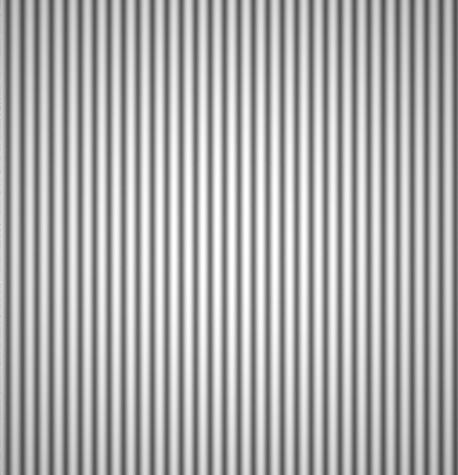
\includegraphics[width=0.3\textwidth]{tifs/tif9.png}
            \label{tif9}}
        \subfigure[]{
            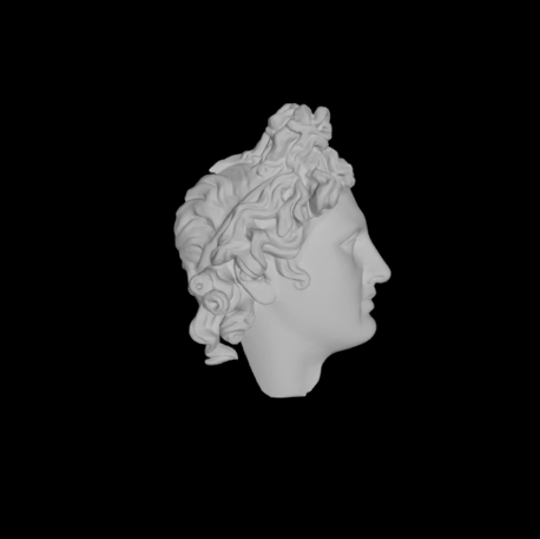
\includegraphics[width=0.3\textwidth]{tifs/tif10.png}
            \label{tif10}}
        \subfigure[]{
            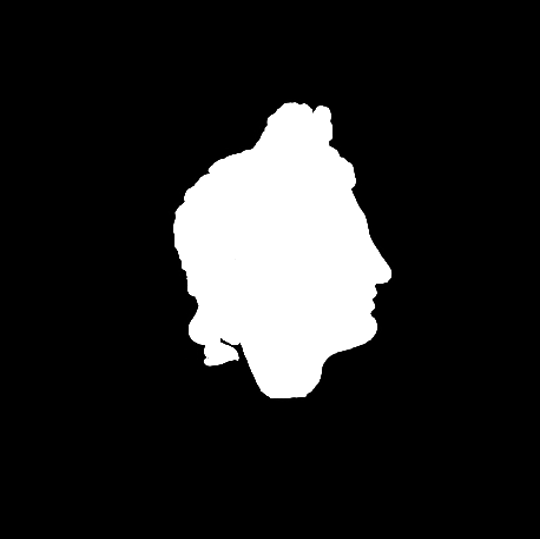
\includegraphics[width=0.3\textwidth]{tifs/tif11.png}
            \label{tif11}}
        \caption{Conjunto de imágenes obtenidos por escena: a), b), c) proyección de franjas con objeto y deslizamiento de fase de $2\pi/3$, d), e), f) proyección de franjas de referencia y deslizamiento de fase de $2\pi/3$, g) Groundtruth, h) Mascara con región de interés.}
        \label{tif456789f1011}
      \end{center}
    \end{figure}
    
\subsection{Extracción de fase y desenvolvimiento de fase}
Una vez obtenidas las imágenes con las franjas proyectadas de el objeto y de referencia, se obtiene el mapa de fase absoluta con la ecuación \ref{absolute_Phase_map} usando el método de 3 pasos (3-Step).

\begin{eqnarray}
\label{absolute_Phase_map}
\phi \left ( x,y \right )= tan^{-1}\left ( \sqrt{3\frac{I_3\left ( x,y \right )-I_1\left ( x,y \right )}{2I_2\left ( x,y \right )-I_1\left ( x,y \right )-I_3\left ( x,y \right )}} \right )
\end{eqnarray}

Las figura \ref{tif1213} muestran un ejemplo de mapa de fase extraído usando la ecuación \ref{absolute_Phase_map}.

\begin{figure}[H]
      \begin{center}
        \subfigure[]{
            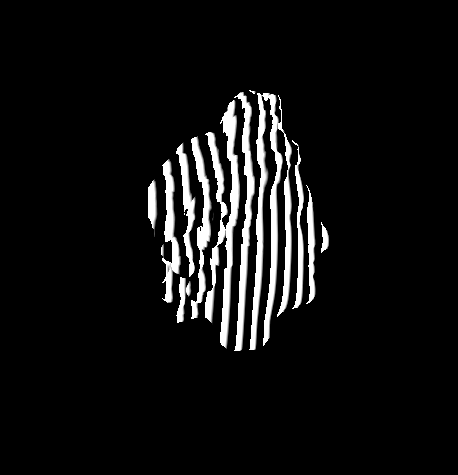
\includegraphics[width=0.4\textwidth]{tifs/tif12.png}
            \label{tif12}}
        \subfigure[]{
            
\includegraphics[width=0.4\textwidth]{tifs/tif13.png}
            \label{tif13}}
        \caption{Mapas de fase objeto y de referencia.}
        \label{tif1213}
      \end{center}
    \end{figure}
    
El desenvolvimiento de fase es el paso mas importante en la reconstrucción 3D. Se han propuesto diversos métodos para realizar esta tarea, sin embargo, en el presente trabajo se utilizo el algoritmo PUMA o cortes gráficos (Cuts Graph)\cite{Biou:Vala}. En este algoritmo, la minimización de energía se logra mediante una secuencia finita de minimizaciones binarias, cada uno logrado de manera eficiente por un flujo máximo/mínimo de corte en ciertos gráficos. El uso de algoritmo PUMA aunque tomaba tiempo obtener la fase desenvuelta, demostró tener el mejor desempeño para obtener mejor información 3D del objeto de estudio. %\textbf{Biou:Vala} 

\begin{figure}[H]
      \begin{center}
        \subfigure[Objeto]{
            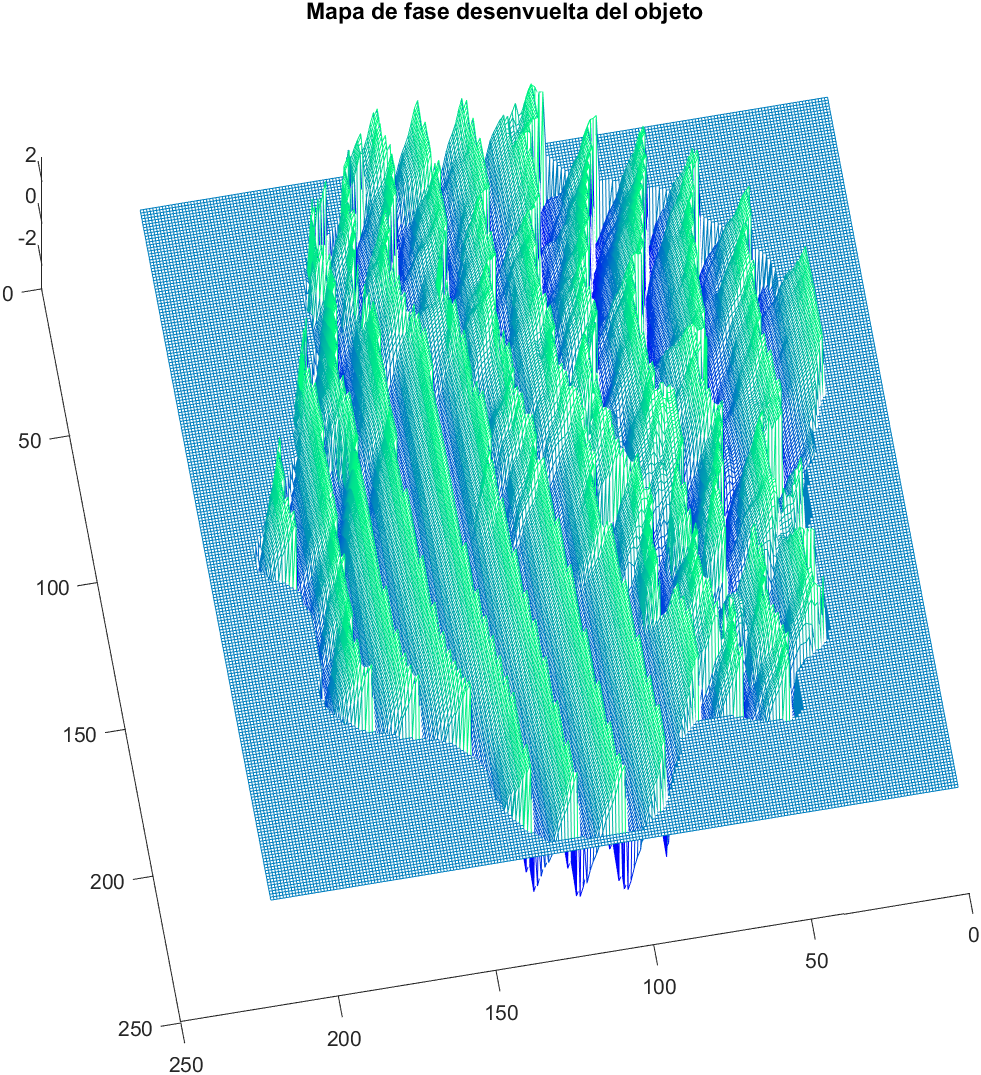
\includegraphics[width=0.4\textwidth]{tifs/tif14.png}
            \label{tif14}}
        \subfigure[Plano de referencia]{
            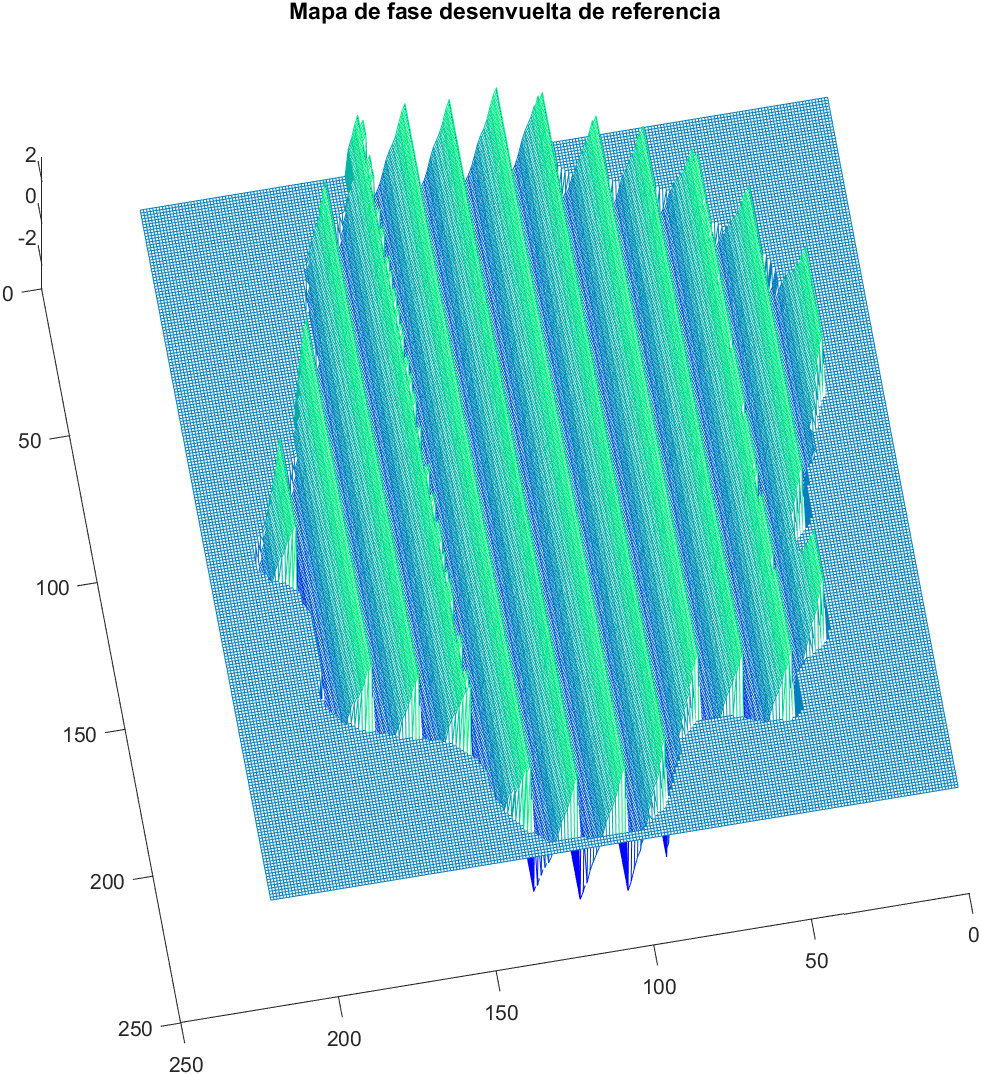
\includegraphics[width=0.4\textwidth]{tifs/tif15.png}
            \label{tif15}}
        \caption{RepresentaciÓn 3D de mapas de fase desenvueltos de objeto y de referencia.}
        \label{tif1415}
      \end{center}
    \end{figure}

\subsection{Filtrado de imágenes}
El mapa absoluto obtenido de las imágenes mediante proyección de franjas muestra un patrón de ruido cuasi/periódico persistente en todas las imágenes obtenidas. Este ruido es producido cuando 2 o mas patrones de franjas periódicos se sobreponen una sobre la otra y es completamente normal que estén presentes en los métodos de deslizamiento de fase. Por lo tanto, como se usan patrones de franjas deslizados para obtener mapas de fase de superficie, estos patrones de ruido periódico o cuasi/periódico (Moire) tienden a estar presentes durante todo el proceso Perfilometría por Deslizamiento de Fase, desde que se obtienen las imágenes hasta que se obtiene el mapa de fase absoluto. El ruido cuasi/periódico es mostrado en la figura \ref{tif16}.

\begin{figure}[H]
	\centering
    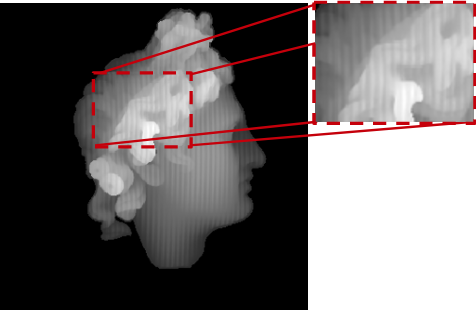
\includegraphics[width=0.5\textwidth]{tifs/tif16.png}
    \caption{Mapa de fase absoluta obtenida mediante la resta de mapa de fase de objeto y de plano de referencia. Se aprecia el ruido cuasi periódico que afecta la reconstrucción 3D del objeto.}
    \label{tif16}
\end{figure}

Este ruido reduce considerablemente la calidad de las reconstrucciones y provoca estimaciones de altura que pueden ser no consistente o poco precisas. Por esta razón, se requiere un procesamiento de la imagen obtenida y corrompida que permita reducir dicho ruido presente. Debido a la dificultad que supone tratar el ruido durante la adquisición de las imágenes o durante el procesamiento para la obtención del mapa de fase absoluto, se propone un paso de pos-procesamiento que consiste en 2 pasos: Proponer un algoritmo que atenué el ruido presente en las imágenes y crear una base de datos con este algoritmo, y procesar mediante una ned neuronal convolucional(CNN) las imágenes procesadas mediante el algoritmo propuesto, esto con el fin de reducir los tiempos de procesamiento de las imágenes afectadas por ruido cuasi/periódico.

\subsubsection{Filtro de umbral adaptable en dominio de la frecuencia y suavizado en dominio espacial}
El desarrollo de un filtro que permita atenuar el ruido de Moire, específicamente el ruido cuasi/periódico, responde a la necesidad de obtener reconstrucciones 3D de alta calidad, por lo que técnicas para el tratamiento de reducción o eliminación del ruido cuasi/periódico en imágenes han ido desarrollándose a lo largo de los años. Así han surgido diversos métodos que tratan de eliminar el ruido de Moire trabajando tanto en el dominio espacial de la imagen como en el dominio de la frecuencia. Bajo esta premisa, Liu(Liu, Yang, \& Yue, 2015)\cite{Liu:Yang} propuso un método de eliminación de patrón Moiré a través de descomposición de matriz dispersa y de rango bajo, sin embargo, esta técnica solo se utiliza exclusivamente cuando los patrones de ruido periódico están bien definidos. Por otro lado, se ha demostrado que el tratamiento del ruido periódico en el dominio de la frecuencia de una imagen corrompida puede dar resultados bastante buenos, de esta forma Varghese(Varghese, 2016)\cite{Varghese:} propone un filtro de umbral adaptable que trabaja en el dominio de la frecuencia de la imagen que se desea eliminar o atenuar el ruido periódico. De esta forma reemplaza los pixeles con frecuencias no deseados con los valores de las frecuencias de la media de sus pixeles vecinos tomando en cuenta un umbral para evitar reemplazar frecuencias validas. Sin embargo, dicho umbral es demasiado alto para algunos casos donde se presenta el ruido de Moire presenta patrones mas irregulares, como los que se presentan cuando el ruido que afecta la imagen es cuasi/periódico. Por otro lado Alvarado (Alvarado, 2020)\cite{Alva:Orte} propone utilizar un filtro de cruz sobre la imagen en el dominio de la frecuencia, con lo que consigue reducir considerablemente el ruido cuasi/periódico en imágenes obtenidas mediante PSP, obteniendo de esta forma reconstrucciones mas suaves y mejores estimaciones de altura en los objetos 3D reconstruidos. %\textbf{Liu:Yang}\textbf{Sun:Yu}

Recientes técnicas hacen uso de redes neuronales convolucionales para eliminar el ruido de Moire. Sun(Sun, Yu, \& Wang, 2018)\cite{Sun:Yu} propone una red neuronal convolucional multiresolución para eliminar el ruido de Moire de imágenes capturadas con cámaras fotográficas de celulares. Sin embargo, dicho patrón de ruido es muy diferente del patrón de ruido obtenido mediante perfilometría de proyección de franjas, por lo que su uso resulta inefectivo para atenuar el ruido de Moire. 

En esta tesis se propone un filtro que atenué el ruido cuasi/periódico en el dominio de la frecuencia en imágenes generadas por perfilometría de franjas, para de esta manera generar una base de datos de imágenes con el cual entrenar una red neuronal convolucional propuesta. Esto con el fin de realizar un pre-procesamiento de imágenes afectadas con ruido en un tiempo reducido como parte de una metodología para la reconstrucción 3D de objetos.

Un filtro de umbral adaptable ademas de un filtro de suavizado es usado para atenuar el ruido presente en las reconstrucciones 3D mediante la atenuación de los pixeles corrompidos con la media de sus pixeles vecinos. Ya que un patrón de franjas verticales es usado para el análisis de franjas, los componentes de ruido normalmente se encontrarían a lo largo de el eje horizontal cuando se analiza la imagen en el dominio de la frecuencia. Sin embargo, dado que las franjas proyectadas sobre el objeto adoptan la forma del mismo, dicho patrón de franjas se distorsiona, por lo que el patrón de ruido que se presenta es cuasi/periódico, por lo tanto se propaga por todo el espectro de la imagen. Un filtro de umbral adaptable se usa para reemplazar directamente los pixeles con las frecuencias corruptas por la media de sus pixeles vecinos, obteniendo de esta forma la frecuencia correspondiente, sin el ruido cuasi/periódico. La figura \ref{tif17} muestra un ejemplo de una imagen en el dominio de la frecuencia con ruido cuasi/periódico en forma de estrella. La figura \ref{tif18} muestra la misma imagen en dominio de la frecuencia con contraste ajustado que resalta prácticamente las frecuencias corrompidas de la imagen. Los pixeles de la región central se excluyen debido a que contienen la mayor información de la imagen, por lo que no son parte del proceso de filtrado. La imagen en la figura \ref{tif19} muestra la imagen original en el dominio de la frecuencia pero con los pixeles corrompidos reemplazados cuando se aplica el filtro de umbral adaptable.

\begin{figure}[H]
      \begin{center}
        \subfigure[Imagen en dominio de frecuencia con ruido cuasi/periódico visible.]{
            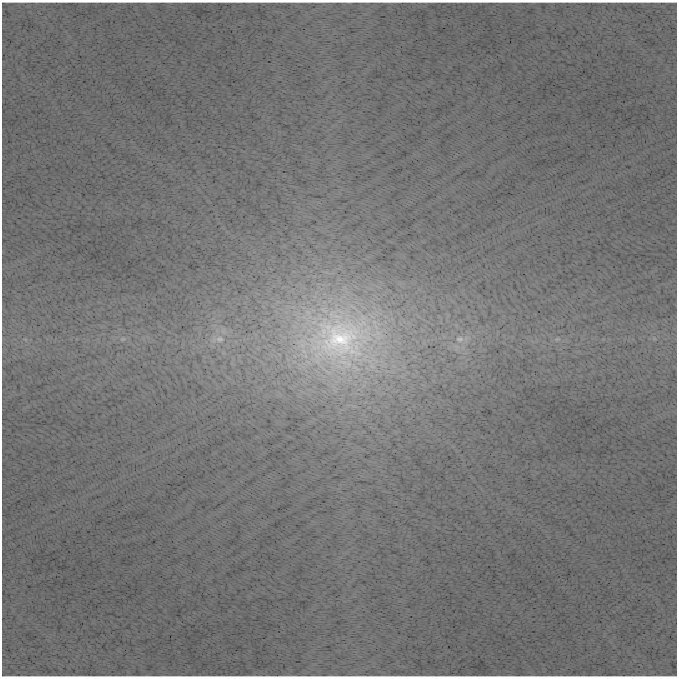
\includegraphics[width=0.3\textwidth]{tifs/tif17.png}
            \label{tif17}}
        \subfigure[Frecuencias no deseadas resaltadas mediante aplicación de contraste a imagen, excluyendo región central.]{
            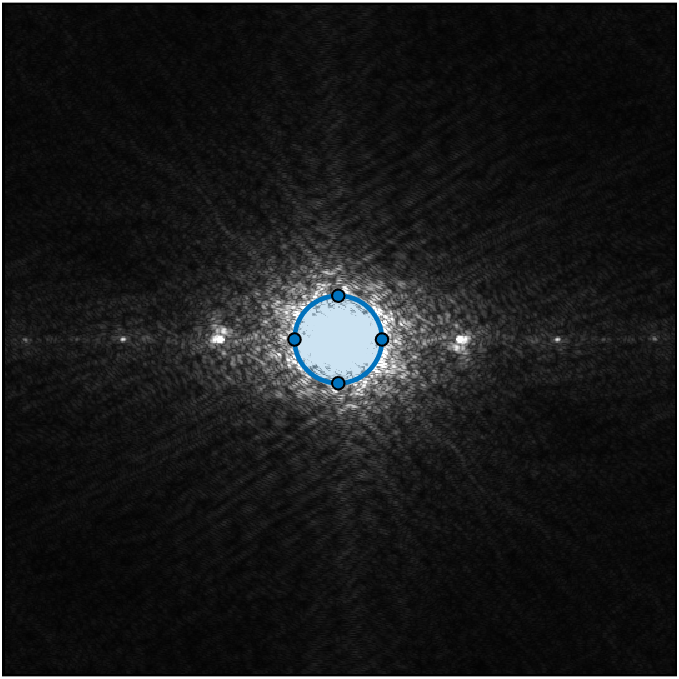
\includegraphics[width=0.3\textwidth]{tifs/tif18.png}
            \label{tif18}}
        \subfigure[Imagen en dominio de frecuencia después de aplicar filtro de umbral adaptativo.]{
            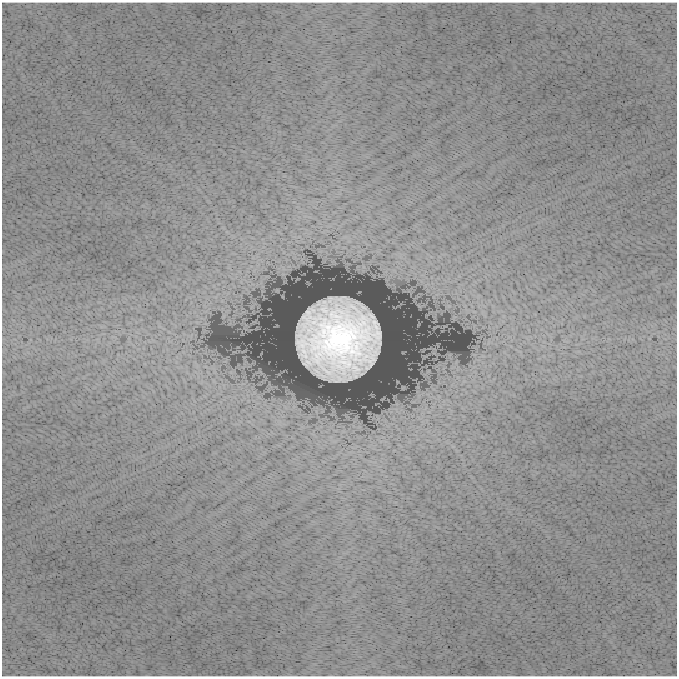
\includegraphics[width=0.3\textwidth]{tifs/tif19.png}
            \label{tif19}}
        \caption{Filtro de umbral adaptativo.}
        \label{tif171819}
      \end{center}
\end{figure}

Dado que el filtro de umbral adaptable trabaja en el dominio de la frecuencia, la imagen que se procesa es convertida a escala de grises, de esta manera se transforma al dominio de la frecuencia mediante transformada rápida de Fourier, después de aplicar el filtro, se reconvierte nuevamente al dominio espacial donde un filtro de suavizado es aplicado para atenuar el ruido residual. La figura \ref{tif22} muestra los pasos para aplicar el filtro de umbral adaptable y filtro de suavizado.

\begin{figure}[H]
	\centering
    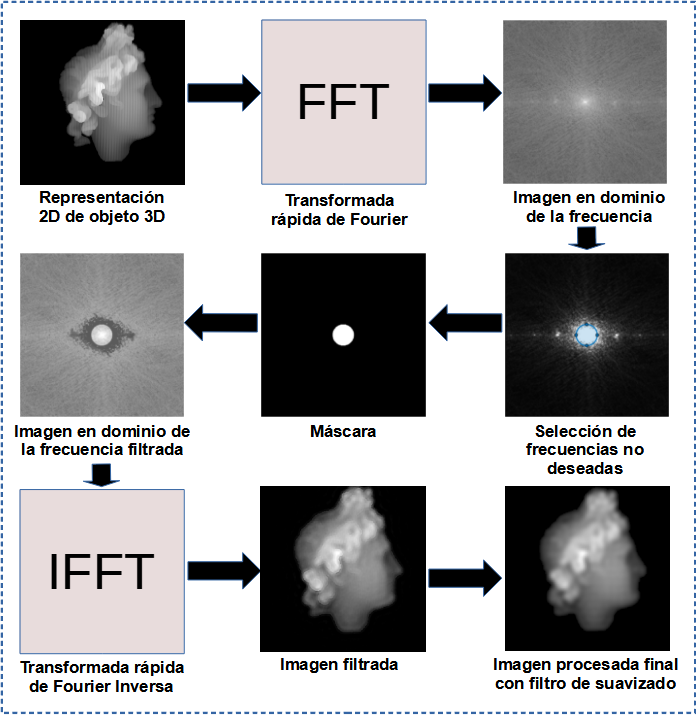
\includegraphics[width=0.8\textwidth]{tifs/tif22.png}
    \caption{Pasos para aplicar filtro adaptable y filtro de suavizado.}
    \label{tif22}
\end{figure}


\subsubsection*{Descripción de algoritmo desarrollado} 
El algoritmo propuesto es una variante del algoritmo ATBF (Adaptive Threshold Based Frequency) creado por Varghese (Varghese, 2016)\cite{Varghese:} que convierte la imagen contaminada con ruido de cuasi/periódico a el dominio de la frecuencia mediante la aplicación de la transformada rápida de Fourier para atenuar el ruido cuasi/periódico mediante la detección de las regiones que lo presentan, reemplazando los pixeles de las regiones localizada con la media del valor de sus pixeles vecinos. Para esto resalta las regiones con ruido y facilitando la detección de pixeles con frecuencias no deseadas. Sin embargo, las frecuencias no deseadas obtenidas mediante proyección de franjas se encuentran generalmente fuera de la región central de la imagen en el dominio de la frecuencia, por lo que se inicia el proceso de filtrado en los extremos superior e inferior de la imagen convergiendo en el centro de la imagen. Debido a que la imagen en su totalidad es procesada, se crea una mascara que contiene las frecuencias originales de la región central donde se encuentra la mayor concentración de información de la imagen para su posterior recuperación cuando termina el procesamiento de la imagen\cite{Espi:Bern}.

El algoritmo desarrollado para atenuar el ruido cuasi/periódico se describe a continuación:

Considerando A como una imagen contaminada con ruido cuasi/periódico de tamaño $m \times n$, se determina F, mostrado en la figura \ref{tif17} de igual tamaño mediante aplicación de transformada de Fourier usando la ecuación \ref{FFT}

\begin{eqnarray}
\label{FFT}
F(u,v)&=&\frac{1}{MN}\sum_{x=0}^{M-1}\sum_{y=0}^{N-1}(-1)^{x+y}A(x,y)e^{-j2\pi(\frac{ux}{M}+\frac{vx}{N})}.
\end{eqnarray}

donde $j^2 = -1$ and $(-1)^{x+y}$ denota el origen de cambio de la operación. Ya que las imágenes contaminadas con ruido cuasi/periódico resaltan en la imagen en el dominio de la frecuencia con forma de estrella, estas regiones pueden ser fácilmente detectadas como se puede apreciar en la figura \ref{tif17}.

\begin{figure}[H]
	\centering
    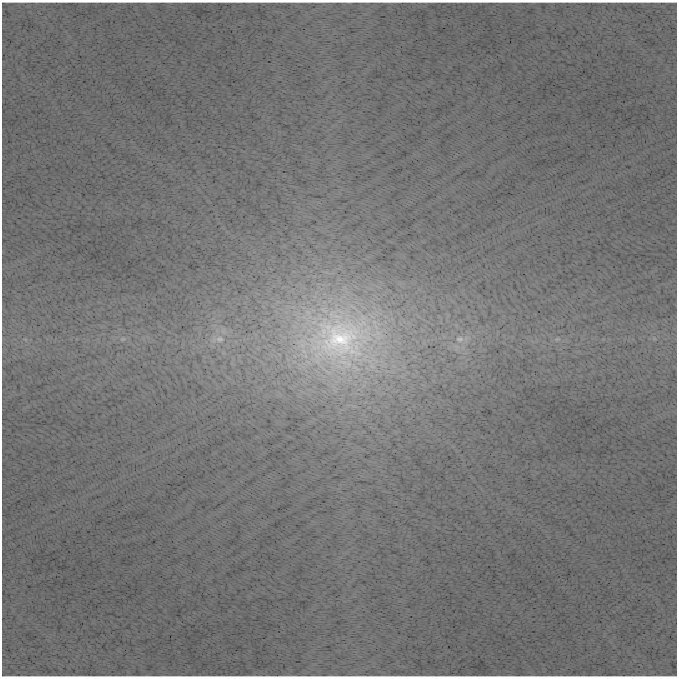
\includegraphics[width=0.4\textwidth]{tifs/tif17.png}
    \caption{Imagen en dominio de frecuencia con ruido de cuasi/periódico visibles.}
    \label{tif17}
\end{figure}

Para resaltar aun mas las regiones que contienen frecuencias no deseadas, se aplica una convolucion con kernel Laplaciano de $5 \times 5$ a la imagen $F$. El kernel utilizado se muestra en la figura \ref{tif24}. Utilizando la ecuación \ref{K5x5}, la operación en la imagen $F$ resulta en la imagen $L$.  

\begin{figure}[H]
	\centering
    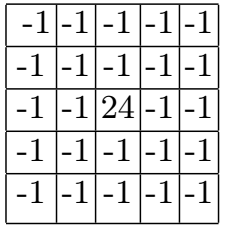
\includegraphics[width=0.3\textwidth]{tifs/tif24.png}
    \caption{Kernel Laplaciano de $5 \times 5$ usado para resaltar regiones con ruido cuasi/periódico.}
    \label{tif24}
\end{figure}

\begin{eqnarray}
\label{K5x5}
L(u,v)&=&\sum_{ker=-2}^{2}\sum_{ker=-2}^{2}F(u+k,v+l)\times K(3+k,3+l).
\end{eqnarray}

La imagen resultante con la operación de convolución con kernel Laplaciano, $L$, se muestra en la figura \ref{tif25}.

\begin{figure}[H]
	\centering
    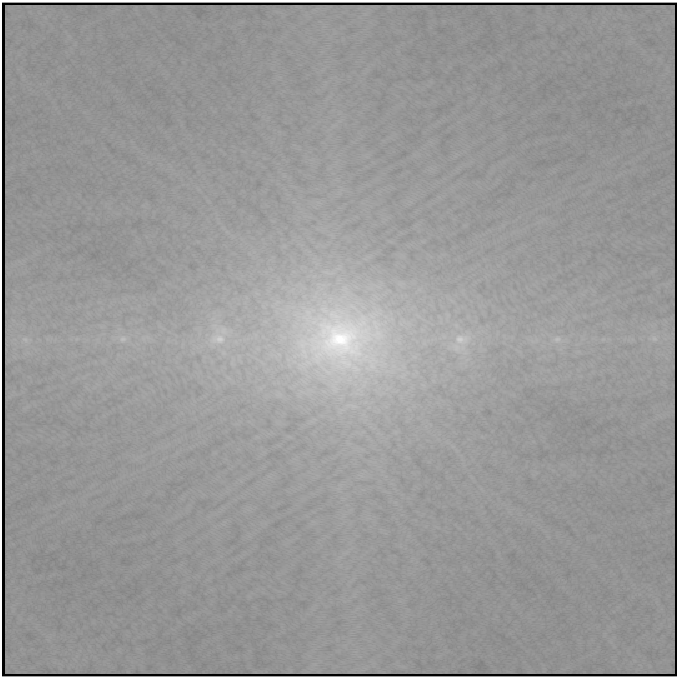
\includegraphics[width=0.4\textwidth]{tifs/tif25.png}
    \caption{Imagen en dominio de frecuencia con ruido cuasi/periódico resaltado mediante aplicación de convolucion con kernel Laplaciano de $5 \times 5$.}
    \label{tif25}
\end{figure}

Después de aplicar convolución Laplaciana, $L$, es procesada para aislar las regiones con ruido aplicando un estiramiento lineal para ajustar contraste de imagen y ajustar los valores de los pixeles a un rango definido por la ecuación \ref{image:stretch}.

\begin{eqnarray}
\label{image:stretch} 
Xnew=\frac{Xinput-Xmin}{Xmax-Xmin}\times 255.
\end{eqnarray}

Los pixeles en $L$ con los valores mas bajos son asignados a 0 mientras que los valores mas altos son asignados a 255. Los demás valores son reasignados de acuerdo con la ecuación \ref{image:stretch}. Este preprocesamiento final sobre la imágenes en el dominio de la frecuencia resulta en $E$, mostrado en la figura \ref{tif26}.

\begin{figure}[H]
	\centering
    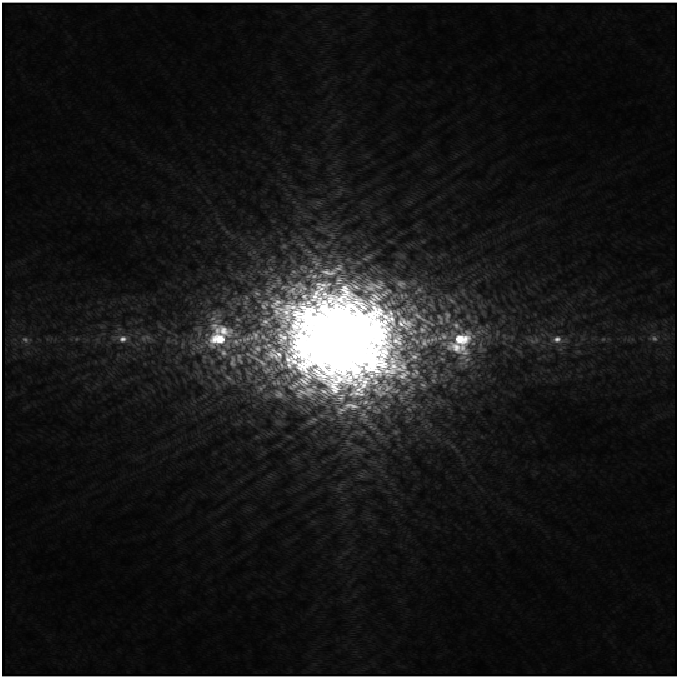
\includegraphics[width=0.4\textwidth]{tifs/tif26.png}
    \caption{Ajuste de contraste para resaltar regiones con ruido cuasi/periódico.}
    \label{tif26}
\end{figure}

\subsubsection*{Etapa de detección y filtrado de picos de frecuencia}

El algoritmo desarrollado para la detección y filtrado de ruido comienza desde la parte superior e inferior de la imagen y procesa fila por fila hasta que convergen en el centro de la imagen para identificar de forma efectiva la regiones con frecuencia no deseadas. El algoritmo sigue los siguientes pasos:

\textit{Paso 1:} Una imagen de tamaño similar que $E$ es creado para obtener ventanas que permitan obtener la media y el máximo de un pixel y sus vecinos para la identificación de regiones con ruido. Imágenes de umbral iniciales $T1 = E$ y $T2 = E$ y una imagen para restauración en el dominio de la frecuencia $F\_th = F$ son definidas. El algoritmo comienza desde la parte superior e inferior de la imagen en las posiciones $E(m = 1, n = 1)$ y $E(m = m, n = 1)$ y termina cuando converge en el centro de la imagen en la posición $E(m/2, n = n)$. Una mascara $maskF$ es creada también formando un elipse de 35 pixeles a partir del centro de la imagen. Como esta región central concentra la mayoría de información de la imagen original es deseable que no resulte afectada.

\textit{Paso 2:} Para cada pixel en la posición $E(row,col)$ se ejecutan los siguientes pasos:

\textit{Paso 2.1:} Para encontrar de manera adaptativa el umbral e identificar regiones con ruido de imagen E, el algoritmo encuentra la media ($Mean$) de los vecinos del pixel que se procesa en la posicion $Mean(T1(row-1 : row+1, col-1 : col+1).*(row-1 : row+1, col-1 : col+1))$ y el máximo ($Maximum$) de los valores de umbral en la posición $Maximum(T1(row - 1 : row + 1, col - 1 : col + 1). * (row - 1 : row + 1, col - 1 : col + 1))$. Un análisis de ($Mean$) y ($Maximum$), se puede concluir lo siguiente:

\textit{Caso 1:}  Si ($Maximum$) corresponde a un pixel con frecuencia no corrompida y su valor es menor que el valor de ($Mean$), entonces ($Maximum$) es la mejor opción para ser el valor del umbral ya que tiene la frecuencia menor.

\textit{Caso 2:} Si ($Maximum$) corresponde a un frecuencia no corrompida y su valor es mayor que ($Mean$), entonces ($Maximum$) es la mejor opción para el valor de umbral.

\textit{Caso 3:} Si ($Maximum$) corresponde a un valor de frecuencia corrompida, entonces ($Mean$) es la mejor selección para el valor de umbral ya que ($Maximum$) evidentemente es un valor muy grande de frecuencia.

Para facilitar la selección del valor de umbral, un parámetro multiplicativo $\alpha$ es incluido para decidir la pureza del estado del valor de la frecuencia en la posición $E(row, col)$ como $T2 = \alpha \times Minimum(m1 ,m2)$. $\alpha$ es un parámetro multiplicativo que es usado para asegurar que la superficie generada por $T$ esta siempre por encima de version contaminada de la imagen $E$.

\textit{Paso 2.2:} Si el valor del pixel en la posición $E(row, col)$ es mas grande que el valor obtenido por el parámetro multiplicativo $\alpha$, es determinado que el valor de la frecuencia en la posición es no deseada y es reemplazado por el valor de sus vecinos en la posición $F\_th(row, col) =
min(min(F th(row - 2 : row + 2, col - 2 : col + 2)))$. De otra forma, el valor en esa posición es conservado como en la imagen original $F\_th(row, col)$.

\textit{Paso 3:} Una vez que todos los pixeles en la fila son procesados, el algoritmo se mueve a la siguiente fila y proceso del paso 2 comienza de nuevo.

\textit{Paso 4:} Si el centro de la imagen $E(ay/2)$ es alcanzado en ambas direcciones, arriba y abajo de la imagen $E$, el algoritmo se termina.

\textit{Paso 5:} Cuando el algoritmo se detiene, la mascara $maskF$ es sumada con la imagen en el dominio de la frecuencia $F\_th$ restaurada. La imagen mostrando las regiones con ruido de $E$ ya restauradas, es mostrada en la figura \ref{tif19}. 

\begin{figure}[H]
	\centering
    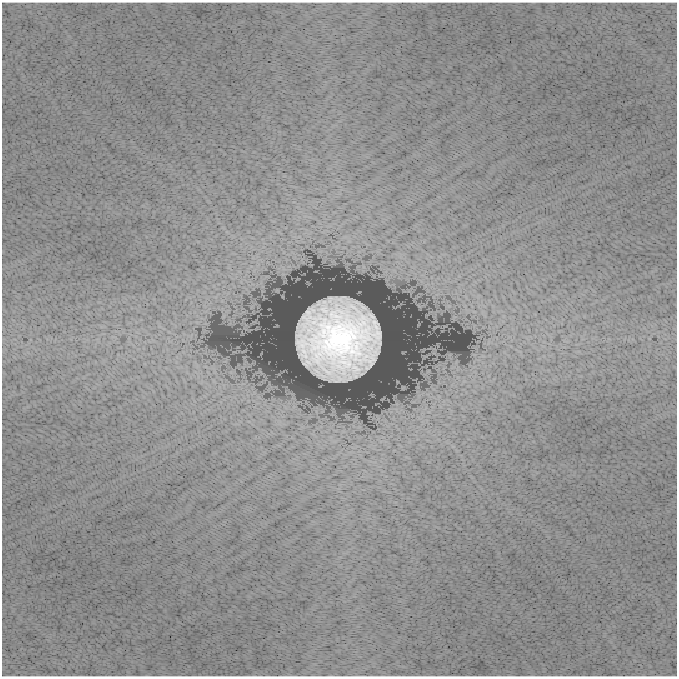
\includegraphics[width=0.4\textwidth]{tifs/tif19.png}
    \caption{Imagen que muestra las regiones identificadas con ruido cuasi/periódico en el dominio de la frecuencia.}
    \label{tif19}
\end{figure}

Una vez que la imagen es $F\_th$ es procesada por el algoritmo de filtrado de ruido, es convertida nuevamente al dominio espacial mediante la transformada inversa de Fourier.

\textit{Paso 6:} Finalmente un filtro de suavizado es aplicado a la imagen convertida al dominio espacial para mejorar la atenuación de las regiones con ruido. El kernel utilizado para esta operación es mostrado en las figuras \ref{tif27} y \ref{tif28}. 

\begin{figure}[H]
      \begin{center}
        \subfigure[]{
            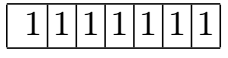
\includegraphics[width=2cm, height=0.4cm]{tifs/tif28.png}
            \label{tif28}}
        \subfigure[]{
            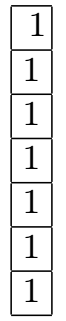
\includegraphics[width=0.4cm, height=2cm]{tifs/tif27.png}
            \label{tif27}}
        \caption{a) $1\times7$ horizontal kernel. b) $1\times7$ vertical kernel.\cite{Gonz:Rich}}
        \label{tif2728}
      \end{center}
    \end{figure}

Una vez que el procesamiento de filtrado de umbral adaptable finaliza, se convierte la imagen nuevamente al dominio espacial. Después un filtro de suavizado es aplicado para mejorar la atenuación de ruido. Finalmente la imagen con el ruido atenuado es mostrado en la figura \ref{tif19} donde se hace una comparación de antes y después del filtrado, con la imagen original \ref{tif29}.

\begin{figure}[H]
      \begin{center}
        \subfigure[]{
            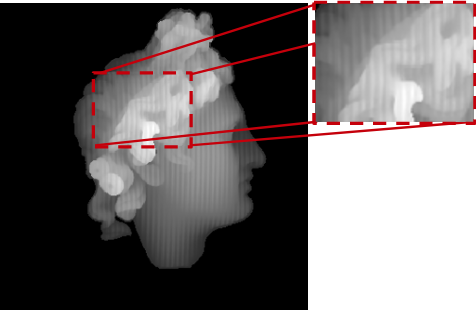
\includegraphics[width=0.46\textwidth]{tifs/tif16.png}
            \label{tif16}}
        \subfigure[]{
            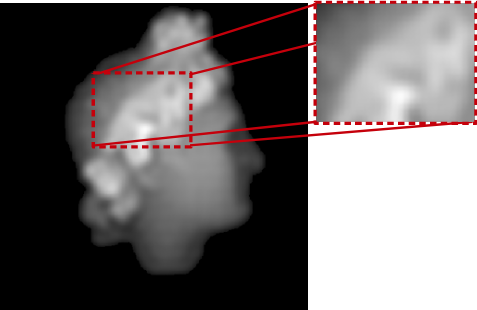
\includegraphics[width=0.46\textwidth]{tifs/tif29.png}
            \label{tif29}}
        \caption{a) Imagen contaminada antes de filtrado. b) Imagen contaminada después de filtrado}
        \label{tif1629}
      \end{center}
    \end{figure}

Pseudocodigo desarrollado e implementado es como sigue:
\\\\
\hrulefill \textit{Read an image \textbf{A}} \\
\hspace*{0.5cm}\textit{A to grayscale}\\
\hspace*{0.5cm}\textit{A to double}\\
\hspace*{0.5cm}\textit{Set ax $\longleftarrow$ Height(A)}\\
\hspace*{0.5cm}\textit{Set ay $\longleftarrow$ Width(A)}\\
\textit{Read \textbf{mask}}\\
\textit{Set A $\longleftarrow$ A.*mask}\\
\textit{Set F $\longleftarrow$ FastFourierTransform(A)}\\
\textit{Obtain image in frequency domain F}\\
\textit{Set f\_laplace5 $\longleftarrow$ Laplacian Kernel 5x5}\\
\textit{Set E $\longleftarrow$ (f\_laplace5(m,n)-min(f\_laplace5)/(max(f\_laplace5)-min(f\_laplace5))*255)}\\
\textit{Set mask $\longleftarrow$ drawellipse('Center',[ax/2 ay/2],'SemiAxes',[35 35]);}	\\
\textit{Set T1 $\longleftarrow$ E}\\
\textit{Set T2 $\longleftarrow$ E}	\\
\textit{Set F\_th $\longleftarrow$ F}\\
\textit{Set maskF $\longleftarrow$ F.*mask}	\\
\textit{Set F\_mask1 $\longleftarrow$ zeros(size(A))}	\\
\textit{Set F\_mask2 $\longleftarrow$ zeros(size(A))}	\\
\textit{Set lim $\longleftarrow$ 3}\\
\textit{Set $\alpha \longleftarrow$ 1.3}: multiplicative factor\\
\textit{Set $\beta \longleftarrow$ 0.3}: umbral above the contaminated image\\
\textit{for row}\\
\hspace*{0.5cm}\textit{for col}\\
\hspace*{1cm}\textit{If E(row,col)$>$(alpha*T2(row,col))}\\
\hspace*{1.5cm}\textit{Reeplaces pixel on F\_th $\longleftarrow$ min(F\_th(row,col))}\\
\hspace*{1cm}\textit{Else}\\
\hspace*{1.5cm}\textit{F\_th(row,col) $\longleftarrow$ F(row,col)}\\
\hspace*{0.5cm}\textit{T1 $\longleftarrow$ T2}\\
\textit{Set F\_filtrado $\longleftarrow$ F\_th + mask}\\
\textit{Set f $\longleftarrow$ InverseFourierTransform(f)}\\
\textit{Set q $\longleftarrow$ q=conv2(f,a17,'same');}\\
\textit{Fin}\\

\subsection{Deep CNN}
El desarrollo de una red neuronal convolucional profunda nos permite entrenar una red neuronal convolucional propuesta para de esta forma automatizar el proceso de filtrado de imágenes con ruido de cuasi/periódico al hacer pasar imágenes a través de un modelo entrenado con las imágenes filtradas mediante el algoritmo propuesto, ahorrando con esto tiempo en el pre-procesamiento durante el proceso de reconstrucción 3D y adquiridas mediante perfilometría de franjas.

Para este fin se desarrollo una variante de la arquitectura de red creada por Sun(Sun, Yu, \& Wang, 2018) \cite{Sun:Yu}. Esta variante agrega 2 capas extras con convolucion de kernel igual a 1 para mantener la arquitectura interna de la red neuronal convolucional original. Ademas se ajusto el tamaño de imágenes para su entrenamiento con un tamaño de $512 \times 512$ diferente del original que entrenaba con tamaños de $256 \times 256$.

Específicamente se agrego una capa de red que permite la entrada y convolución de imágenes con un(1) solo canal y una salida de un canal(1), como se observa en la figura \ref{}, ya que la red Multiresolution-CNN creada por Sun(Sun, Yu, \& Wang, 2018) \cite{Sun:Yu}, admite imágenes de 3 canales y proporciona un salida similar.

\begin{figure}[H]
	\centering
    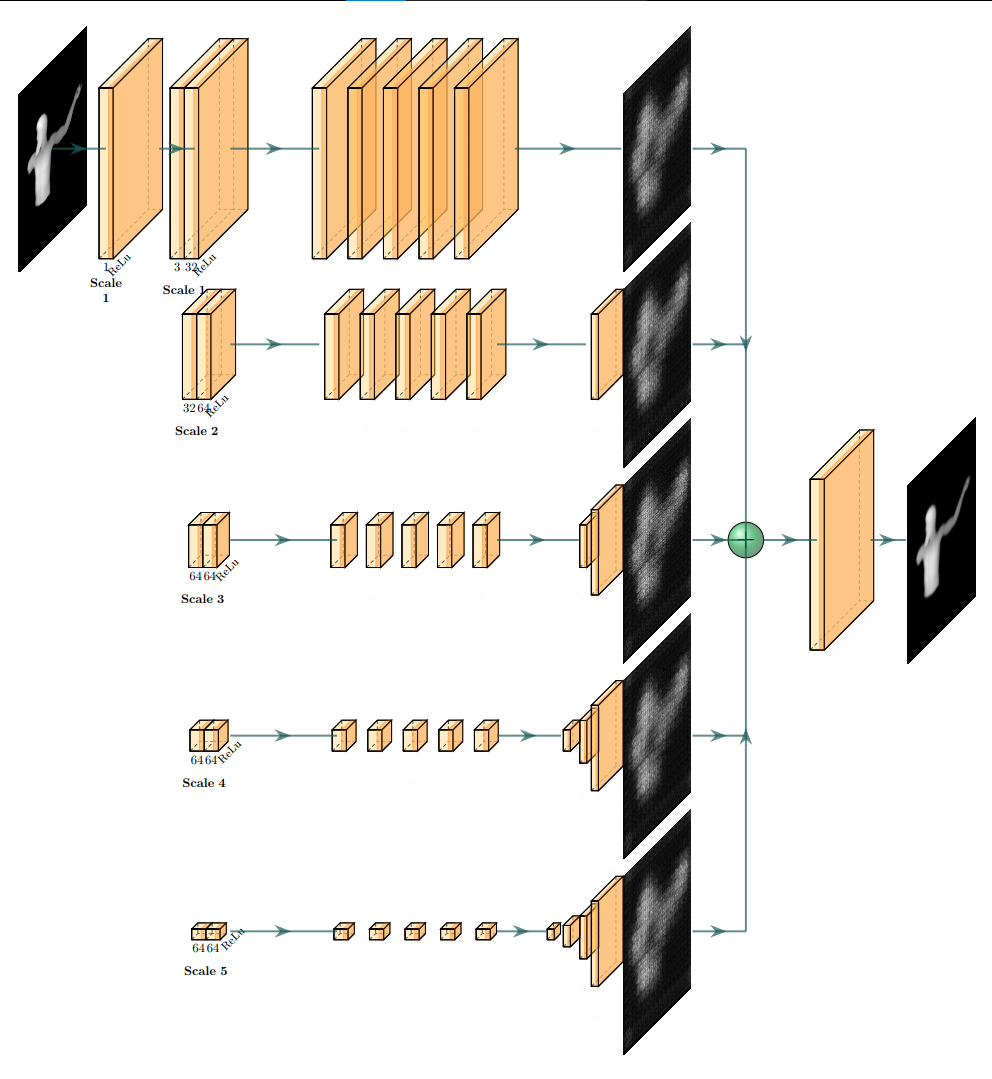
\includegraphics[width=0.8\textwidth]{tifs/tif23.png}
    \caption{Arquitectura propuesta de red neuronal convolucional profunda.}
    \label{tif23}
\end{figure}

Las configuraciones de la red usadas en cada capa se muestran en las tablas \ref{Down:} y \ref{Up:}.

\begin{table}[H]
\begin{center}
\begin{tabular}{ c  c  c  c  c }
\hline
Scale & Type & Kernel & Stride & Channels\\	
\hline
1 & conv & 1x1 & 1x1 & 1 \\
\hline
1 & conv & 3x3 & 1x1 & 3 \\
\hline
1 & conv & 3x3 & 1x1 & 64 \\
1 & conv & 3x3 & 1x1 & 64 \\
\hline
2 & conv & 3x3 & 2x2 & 128 \\
2 & conv & 3x3 & 1x1 & 128 \\
\hline
3 & conv & 3x3 & 2x2 & 256 \\
3 & conv & 3x3 & 1x1 & 256 \\
\hline
4 & conv & 3x3 & 2x2 & 512 \\
4 & conv & 3x3 & 1x1 & 512 \\
\hline
5 & conv & 3x3 & 2x2 & 1024 \\
5 & conv & 3x3 & 1x1 & 1024 \\
\hline
\end{tabular}
\caption{Capas de convolución}
\label{Down:}
\end{center}
\end{table}

\begin{table}[H]
\begin{center}
\begin{tabular}{ c  c  c  c  c }
\hline
Scale & Type & Kernel & Stride & Channels\\	
\hline
1 & conv    & 1x1 & 1x1 & 1 \\
\hline
1 & conv    & 3x3 & 1x1 & 3 \\
\hline
2 & deconv  & 4x4 & 2x2 & 128 \\
  & conv    & 3x3 & 1x1 & 64 \\
  & conv    & 3x3 & 1x1 & 64 \\
\hline
3 & deconv  & 4x4 & 2x2 & 256 \\
  & conv    & 3x3 & 1x1 & 128 \\
  & conv    & 3x3 & 1x1 & 128 \\
\hline
4 & deconv  & 4x4 & 2x2 & 512 \\
  & conv    & 3x3 & 1x1 & 256 \\
  & conv    & 3x3 & 1x1 & 256 \\
\hline
5 & deconv  & 4x4 & 2x2 & 1024 \\
  & conv    & 3x3 & 1x1 & 512 \\
  & conv    & 3x3 & 1x1 & 512 \\
\hline
\end{tabular}
\caption{Capas de deconvolución}
\label{Up:}
\end{center}
\end{table}

%En anexos se puede encontrar la arquitectura de la red propuesta con mas detalle.


\section{RESULTADOS}
Los resultados son presentados en tres secciones diferentes siendo la primera sección la generación de la base de datos, la segunda sección los resultados obtenidos aplicando el algoritmo propuesto y desarrollado con las imágenes obtenidas de la base de datos creada y su reconstrucción final. Finalmente se tienen los resultados obtenidos del entrenamiento de una red neuronal convolucional con la base de datos generada y como afecta la reconstrucción 3D final de los objetos. El desarrollo del entorno de emulación del sistema de perfilometría de franjas se realiza en un ordenador personal con un procesador I7-10750H de @2.60 GHz, con 16 Gb de memoria RAM y una tarjeta gráfica NVIDIA GeForce RTX 3060 con 6 Gb de memoria RAM. Los experimentos y pruebas se realizan también con el equipo mencionado y Matlab 2020a.

\subsection{Base de datos de imágenes}
La imágenes creadas fueron capturadas por un sistema emulado utilizando el software libre \textit{Blender} version 2.95.5.. El proyector es representado por una lampara que proyecta franjas. La cámara tiene una longitud focal de 28 mm. Los modelos de objetos 3D son adquiridos de plataformas en linea como \textit{TurboSquid} que también son de uso libre.

En la imágenes de la figura \ref{imagenesBasedata} muestra algunas imágenes generadas para crear la base de datos. Algunos objetos muestran una superficie parecida al rostro humano por lo que fueron seleccionados para conformar la base datos. Otros objetos fueron seleccionados por su forma geométrica para apreciar mejor los resultados. Finalmente se escogieron algunos con relieve complejo para observar su comportamiento y rendimiento al momento de reconstruirlos y agregar variedad a la base de datos para el entrenamiento de la red neuronal convolucional.

\begin{figure}[H]
      \begin{center}
        \subfigure[]{
            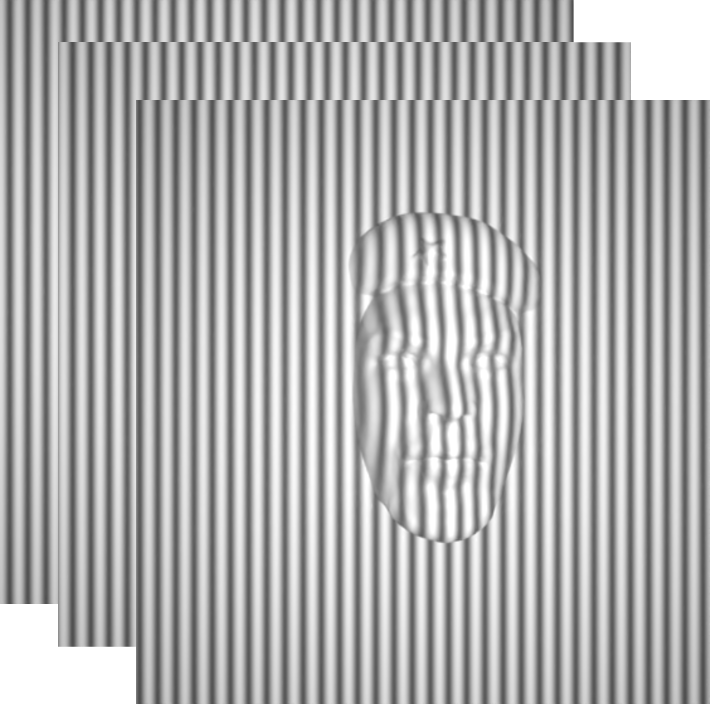
\includegraphics[width=0.3\textwidth]{tifs/tif40.png}
            \label{tif40}}
        \subfigure[]{
            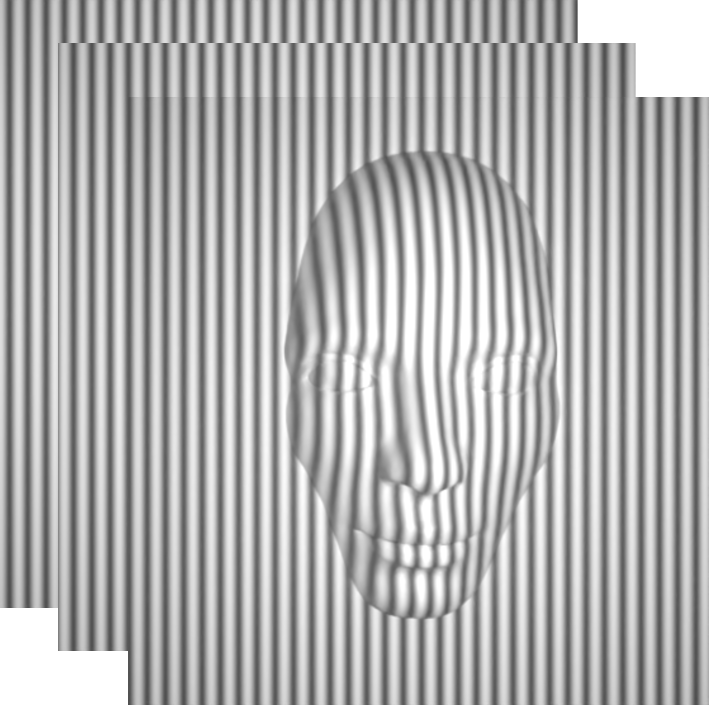
\includegraphics[width=0.3\textwidth]{tifs/tif41.png}
            \label{tif41}}
        \subfigure[]{
            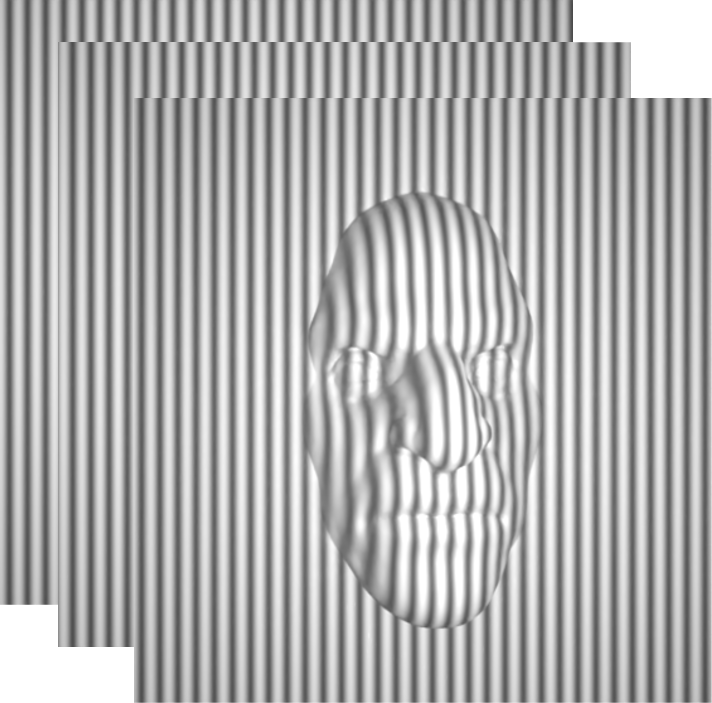
\includegraphics[width=0.3\textwidth]{tifs/tif42.png}
            \label{tif42}}
        \subfigure[]{
            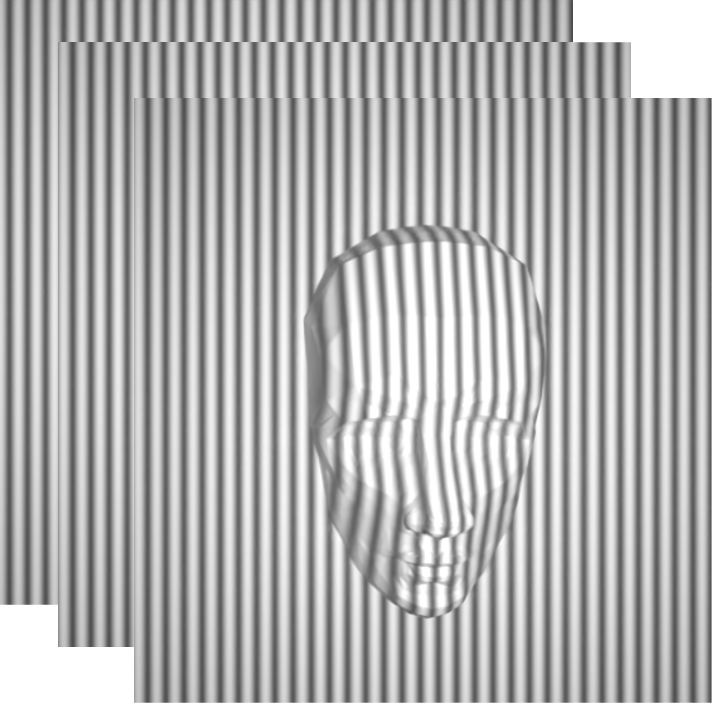
\includegraphics[width=0.3\textwidth]{tifs/tif43.png}
            \label{tif43}}
        \subfigure[]{
            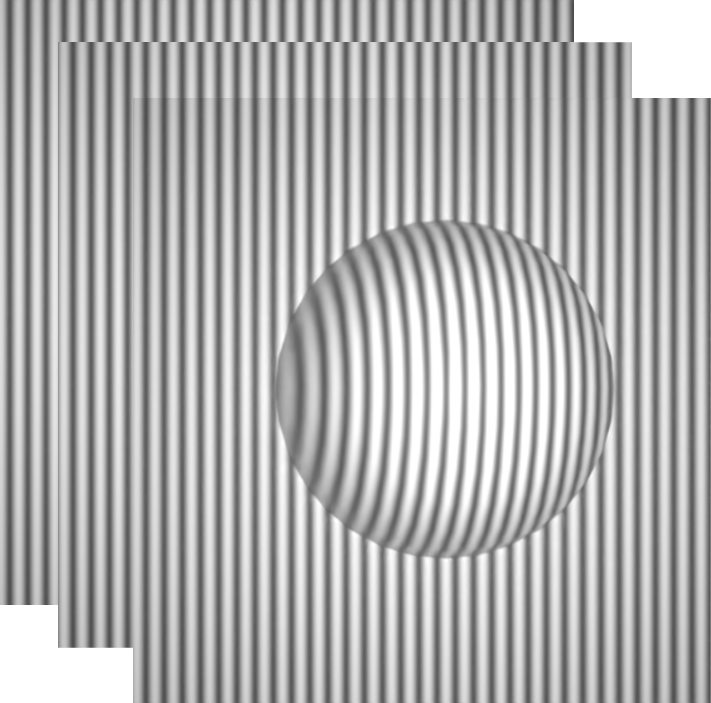
\includegraphics[width=0.3\textwidth]{tifs/tif44.png}
            \label{tif44}}
        \subfigure[]{
            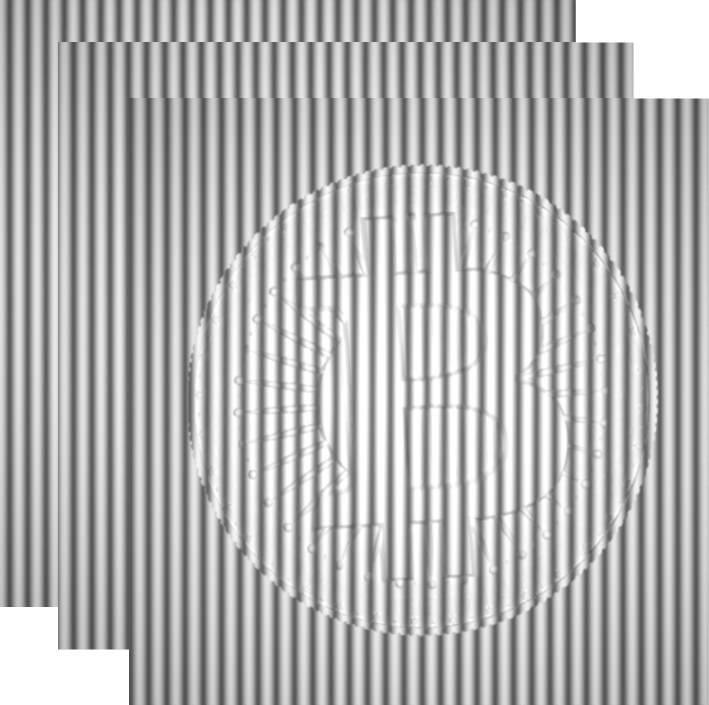
\includegraphics[width=0.3\textwidth]{tifs/tif45.png}
            \label{tif45}}
        \subfigure[]{
            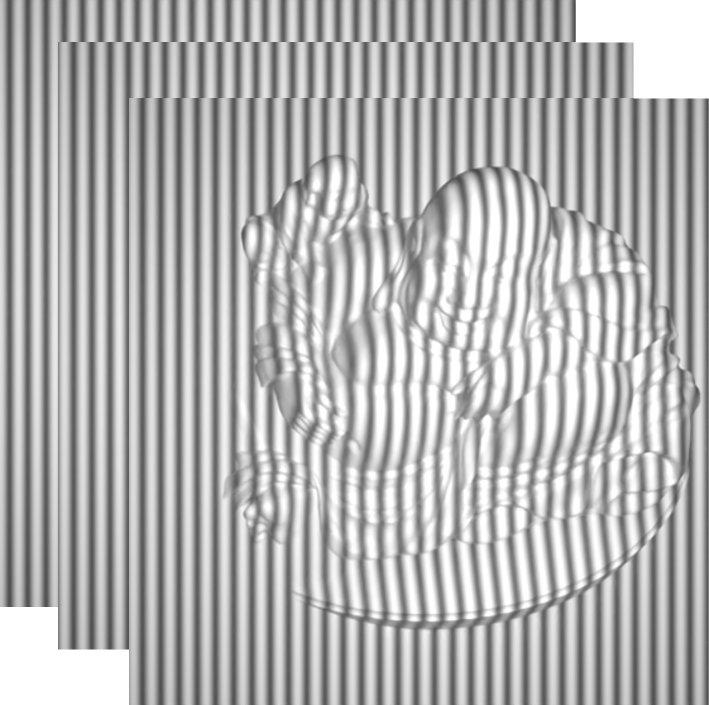
\includegraphics[width=0.3\textwidth]{tifs/tif46.png}
            \label{tif46}}
        \subfigure[]{
            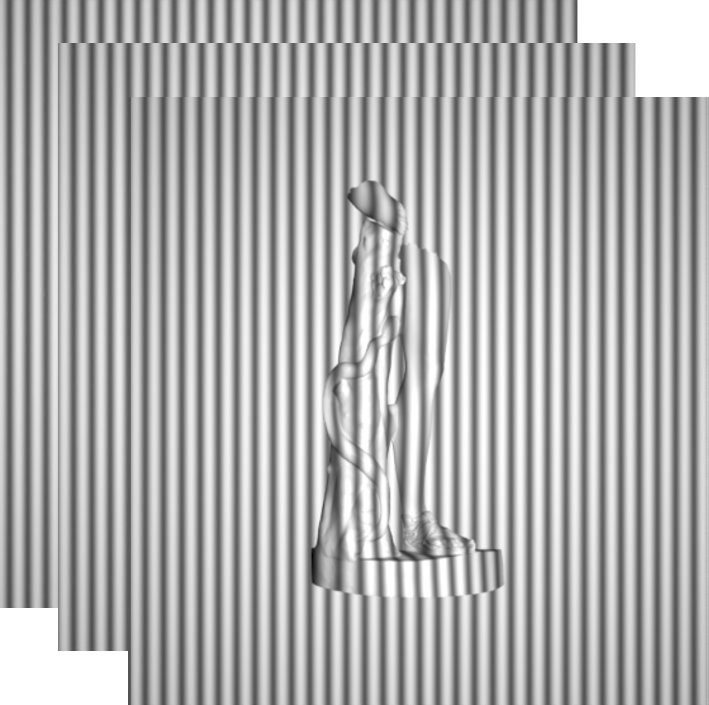
\includegraphics[width=0.3\textwidth]{tifs/tif47.png}
            \label{tif47}}
        \subfigure[]{
            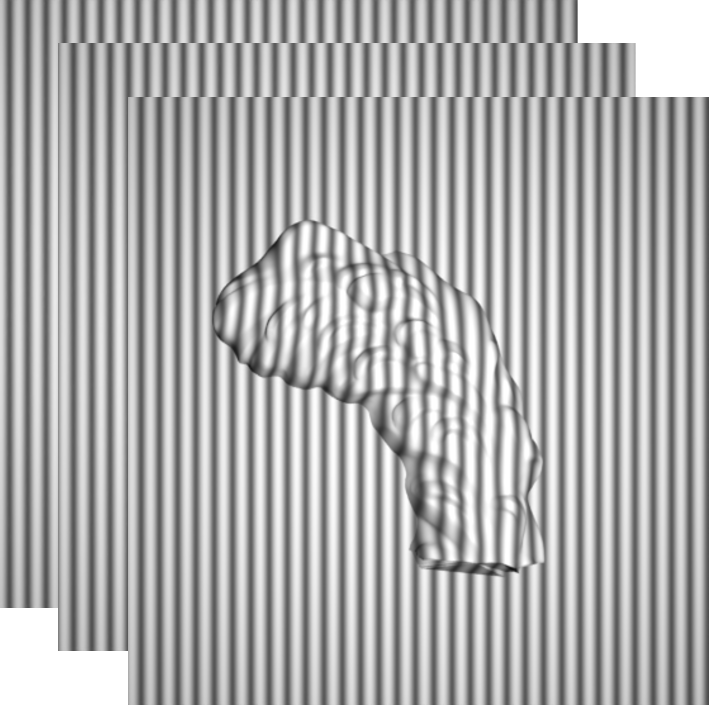
\includegraphics[width=0.3\textwidth]{tifs/tif48.png}
            \label{tif48}}
        \caption{Conjunto de imágenes generados para creación de base de datos.}
        \label{imagenesBasedata}
      \end{center}
    \end{figure}
    
Las imágenes de la figura \ref{imagenesBasedata} muestran algunos objetos utilizados con proyección de franjas en conjuntos de 3 imágenes requeridos en el método de perfilometría de cambio de fase de 3 pasos (3-Step). En total se obtuvieron 345 escenas diferentes con proyección de franjas sumando un total de 1035 imágenes con franjas proyectadas.

Ademas también se crearon 3 mapas de referencia por escena generando 1035 imágenes también. Finalmente se creo una imagen con el objeto real 3D, 345 en total y una imagen mascara que contiene la región de interés del objeto, 345 en total, totalizando 2760 imágenes, que componen la base de datos. Los mapas de referencia, del objeto original y la mascara de la región de interés son mostrados en la figura \ref{tif456789f1011}.

\subsection{Reconstrucciones 3D con algoritmo desarrollado}
Los resultados del algoritmo desarrollado puede observase en la imágenes de la figura \ref{tif49505152}, que siguen la metodología utilizada implementado el algoritmo de filtro de umbral adaptativo desarrollado. Las imágenes de las figuras \ref{tif52} y \ref{tif49} muestran el objeto 3D original y la mascara con la región de interés del objeto. En esta imágenes se puede apreciar el resultado obtenido al usar un objeto con la apariencia del rostro humano, esto para fines de aplicación de reconocimiento facial. En la imagen de la figura \ref{tif50} puede apreciarse claramente como se reduce significativamente el ruido de cuasi/periódico comparado con la imagen de la figura \ref{tif51}. Se obtiene una representación 2D del objeto 3D con mas ausencia de ruido cuasi/periódico.

\begin{figure}[H]
      \begin{center}
        \subfigure[Superficie de objeto original.]{
            \includegraphics[width=0.3\textwidth]{tifs/tif49.png}
            \label{tif49}}
        \subfigure[Mascara de región de interés.]{
            \includegraphics[width=0.3\textwidth]{tifs/tif52.png}
            \label{tif52}}
        \subfigure[Reconstrucción 2D usando PSP.]{
            \includegraphics[width=0.3\textwidth]{tifs/tif51.png}
            \label{tif51}}
        \subfigure[Reconstrucción 2D usando PSP y filtro adaptativo.]{
            \includegraphics[width=0.3\textwidth]{tifs/tif50.png}
            \label{tif50}}
        \caption{Reconstrucción de objeto 3D por etapas en visualización 2D.}
        \label{tif49505152}
      \end{center}
    \end{figure}


La imágenes de la figura \ref{tif535455} muestra la representación 3D de la reconstrucción del objeto mostrado en la figura \ref{tif49505152} después de aplicar un escalamiento que ajusta las alturas mediante minimización de error cuadrático medio \cite{Alfa:Mont} para poder realizar la comparación. Con este escalamiento se puede realizar la comparación del objeto 3D original y el objeto 3D obtenido después de aplicar el algoritmo de filtrado propuesto. Aquí se puede apreciar mejor como el algoritmo desarrollado reduce el ruido cuasi/periódico produciendo un objeto 3D reconstruido con una superficie mas suave y por tanto, mas aproximado al objeto real. %\textbf{Alfa:Mont}

\begin{figure}[H]
      \begin{center}
        \subfigure[Reconstrucción 3D usando PSP.]{
            \includegraphics[width=0.3\textwidth]{tifs/tif53.png}
            \label{tif53}}
        \subfigure[Reconstrucción 3D usando PSP y Filtro Adaptativo.]{
            \includegraphics[width=0.3\textwidth]{tifs/tif54.png}
            \label{tif54}}
        \subfigure[Reconstrucción 3D de Objeto Original.]{
            \includegraphics[width=0.3\textwidth]{tifs/tif55.png}
            \label{tif55}}
        \caption{Reconstrucción de objeto 3D.}
        \label{tif535455}
      \end{center}
\end{figure}
    
\subsection{Filtro adaptativo y filtro de suavizado visto de cerca}
El resultado de aplicar el filtro desarrollado aplicado en el dominio de la frecuencia ademas de un filtro de suavizado con kernel Laplaciano de $5 \times 5$ permite remover significativamente el ruido cuasi/periódico generado por el efecto de Moire producido durante la proyección de un patrón de franjas sobre un objeto 3D. Esto puede apreciarse claramente en las imágenes de la figura \ref{tif5657} ademas de la reconstrucción 3D del objeto mostrado en la figura \ref{tif535455}. Se puede apreciar que la perdida de información del objeto que se desea reconstruir es mínima por lo tanto muy aproximado al objeto real.

\begin{figure}[H]
      \begin{center}
        \subfigure[Reconstrucción 3D usando PSP.]{
            \includegraphics[width=0.45\textwidth]{tifs/tif56.png}
            \label{tif56}}
        \subfigure[Reconstrucción 3D usando PSP y Filtro Adaptativo.]{
            \includegraphics[width=0.45\textwidth]{tifs/tif57.png}
            \label{tif57}}
        \caption{Una vista cercana al ruido cuasi/periódico tratado con el filtro adapatativo desarrollado mas filtro de suavizado.}
        \label{tif5657}
      \end{center}
\end{figure}

La imagen de la figura \ref{tif58} muestra el análisis de perfil del objeto mostrado anteriormente. Se puede apreciar como el perfil del objeto 3D tratado con el filtro adaptativo y de suavizado(representado por linea verde) muestra un perfil mas suave por lo que se aproxima mejor al objeto 3D real reconstruido. Ademas se puede apreciar como el ruido de Moire presente en el perfil del objeto 3D sin aplicación del filtro desarrollado(representado por linea roja) muestra variaciones de reconstrucción bastante grandes, ademas, es representativo de una imagen afectada por ruido periódico o cuasi/periódico, por lo que presenta una reconstrucción con error muy grande de superficie cuando se compara con el objeto 3D original.

\begin{figure}[H]
	\centering
    \includegraphics[height=6cm,width=12cm]{tifs/tif58.png}
    \caption{Análisis de perfil de objeto 3D reconstruido antes y después de aplicar filtro adaptativo desarrollado y suavizado desarrollado.}
    \label{tif58}
\end{figure}

\subsection{Entrenamiento de Red Neuronal Convolucional Profunda (Deep CNN)}

Para realizar el entrenamiento de la red neuronal propuesta, se utiliza la base de datos generada con software \textit{Blender}, en el que se pre-procesaron las imágenes con ruido cuasi/periódico una vez que se le aplico la extracción y desenvolvimiento de fase usando el algoritmo desarrollado mostrado en la sección 4.2, esto para obtener las imágenes objetivo(target) de cada imagen afectada por ruido cuasi/periódico. Este entrenamiento se realizo en un ordenador personal con un procesador I7-10750H de @2.60 GHz, con 16 Gb de memoria RAM y una tarjeta gráfica NVIDIA GeForce RTX 3060 Laptop GPU con 6 Gb de memoria RAM. Se uso también el software Python 3.7.11, libreria Pytorch 1.9.0, y entorno de programación PyCharm Community Edition 2021.1.1.. 
%Ademas también se uso una tarjeta gráfica NVIDIA GeForce GTX 1070 para comparación.

Para realizar el entrenamiento se dividieron las 345 imágenes en proporción de 70\% para entrenamiento, 10\% para validación y 20\% para pruebas siguiendo la metodología propuesta por Sun(Sun, Yu, \& Wang, 2018)\cite{Sun:Yu}. Algunas imágenes de la base de datos pueden observarse en la figura \ref{tif59606162636465666768f69} tanto la imagen con ruido cuasi/periódico como su correspondiente imagen objetivo pre-procesada con el algoritmo desarrollado para atenuar el ruido cuasi/periódico.

Se puede observar la amplia variedad de imágenes utilizadas para el entrenamiento, esto con el fin de tener una variedad al realizar el entrenamiento y hacer una generalización mayor al filtrar tanto objetos 3D simples como objetos 3D complejos.

\begin{figure}[H]
      \begin{center}
        \subfigure[Imagen con ruido.]{
            \includegraphics[height=2.2cm,width=2.2cm]{tifs/tif59.png}
            \label{tif59}}
        \subfigure[Imagen filtrada.]{
            \includegraphics[height=2.2cm,width=2.2cm]{tifs/tif64.png}
            \label{tif65}}
        \subfigure[Imagen con ruido.]{
            \includegraphics[height=2.2cm,width=2.2cm]{tifs/tif60.png}
            \label{tif59}}
        \subfigure[Imagen filtrada.]{
            \includegraphics[height=2.2cm,width=2.2cm]{tifs/tif65.png}
            \label{tif65}}
        \subfigure[Imagen con ruido.]{
            \includegraphics[height=2.2cm,width=2.2cm]{tifs/tif61.png}
            \label{tif61}}
        \subfigure[Imagen filtrada.]{
            \includegraphics[height=2.2cm,width=2.2cm]{tifs/tif66.png}
            \label{tif66}}
        \subfigure[Imagen con ruido.]{
            \includegraphics[height=2.2cm,width=2.2cm]{tifs/tif62.png}
            \label{tif62}}
        \subfigure[Imagen filtrada.]{
            \includegraphics[height=2.2cm,width=2.2cm]{tifs/tif67.png}
            \label{tif67}}
        \subfigure[Imagen con ruido.]{
            \includegraphics[height=2.2cm,width=2.2cm]{tifs/tif63.png}
            \label{tif63}}
        \subfigure[Imagen filtrada.]{
            \includegraphics[height=2.2cm,width=2.2cm]{tifs/tif68.png}
            \label{tif68}}
        \subfigure[Imagen con ruido.]{
            \includegraphics[height=2.2cm,width=2.2cm]{tifs/tif69.png}
            \label{tif69}}
        \subfigure[Imagen filtrada.]{
            \includegraphics[height=2.2cm,width=2.2cm]{tifs/tif70.png}
            \label{tif70}}
        \caption{Imágenes de base de datos generada para entrenamiento de Red Neuronal Convolucional (CNN).}
        \label{tif59606162636465666768f69}
      \end{center}
\end{figure}

El entrenamiento de la red propuesta fue realizado en 00:44:48 horas alcanzando una perdida por entrenamiento(Train Loss) de 6.4e-5 y una perdida por validación (\textbf{Val Loss}) de 0.000127, como se muestra en la gráfica de la figura \ref{tif71}..

\begin{figure}[H]
	\centering
    \includegraphics[height=5cm,width=12cm]{tifs/tif71.png}
    \caption{Evolución de la perdida de validación(\textbf{Loss Val}).}
    \label{tif71}
\end{figure}

%\begin{figure}[H]
%	\centering
%    \includegraphics[width=1\textwidth]{tifs/tif72.png}
%    \caption{Evolución de la perdida(\textbf{Loss}).}
%    \label{tif72}
%\end{figure}

Como resultado de aplicar la red neuronal entrenada con imágenes con representación 2D de objetos que contienen ruido cuasi/periódico, se muestra una atenuación del ruido cuasi/periódico en imágenes adquiridas mediante perfilometría de franjas. Esto puede apreciarse en las imágenes de la figura \ref{tif7980} donde se muestra un objeto representado en 2D del conjunto de pruebas utilizado para probar la red desarrollada e implementada. Se puede apreciar en la imagen aumentada \ref{tif79} la presencia de ruido cuasi/periódico en la imagen del objeto 3D mientras que en la imagen de la figura \ref{tif80} se muestra la ausencia del ruido de cuasi/periódico. Después de la inferencia realizada se realiza un perfilado a la imagen con el fin de resaltar los bordes y detalles de la imagen con el objeto 3D con una convolución con kernel Laplaciano de $[0\; -1\; 0;-1\; 4\; -1; 0\; -1\; -0]$ y un kernel identidad de $[0\; 0\; 0; 0\; 1\; 0; 0\; 0\; 0]$.

\begin{figure}[H]
      \begin{center}
        \subfigure[Objeto]{
            \includegraphics[width=0.45\textwidth]{tifs/tif79.png}
            \label{tif79}}
        \subfigure[Plano de referencia]{
            \includegraphics[width=0.45\textwidth]{tifs/tif80.png}
            \label{tif80}}
        \caption{Vista cercana del ruido de Moire procesado con la red neuronal convolucional desarrollada (Multiresolution CNN Modified).}
        \label{tif7980}
      \end{center}
    \end{figure}

La imagen de la figura \ref{tif818283} muestra la reconstrucción 3D del objeto utilizado en la figura \ref{tif7980}, en el que se le aplica un escalamiento de alturas para su comparación con el objeto original\cite{Alfa:Mont}. Se puede apreciar como el pre-procesamiento realizado con la red neuronal convolucional(Multiresolution-CNN Modified) atenúa completamente el ruido cuasi/periódico presente en la imagen, produciendo un objeto 3D reconstruido mas suave en su superficie y aproximado al objeto real.

\begin{figure}[H]
      \begin{center}
        \subfigure[Reconstrucción 3D usando PSP.]{
            \includegraphics[width=0.3\textwidth]{tifs/tif82.png}
            \label{tif82}}
        \subfigure[Reconstrucción 3D usando PSP y Multiresolution-CNN Modified.]{
            \includegraphics[width=0.3\textwidth]{tifs/tif83.png}
            \label{tif83}}
        \subfigure[Reconstrucción 3D de Objeto Original.]{
            \includegraphics[width=0.3\textwidth]{tifs/tif81.png}
            \label{tif81}}
        \caption{Reconstrucción de objeto 3D.}
        \label{tif818283}
      \end{center}
\end{figure}

Un análisis posterior mostrado en la figura \ref{tif84} muestra el perfil del objeto 3D reconstruido a partir de la representación 2D procesada con la red Multiresolution-CNN Modified mostrado anteriormente. Se aprecia como el perfil del objeto 3D obtenido con la red entrenada produce un perfil mas suave comparado con el objeto con ruido cuasi/periódico original, por lo que su reconstrucción es mas suave, y por tanto mas cercano al objeto original.  

\begin{figure}[H]
	\centering
    \includegraphics[width=1\textwidth]{tifs/tif84.png}
    \caption{Análisis de perfil de objeto 3D reconstruido antes y después de pre-procesamiento con Multiresolution-CNN Modified.}
    \label{tif84}
\end{figure}

\subsection{Comparación con otras arquitecturas}
La metodologia propuesta presentada en este trabajo se basa en una version modificada de la red neuronal convolucional propuesta por Sun (Sun, Yu, \& Wang, 2018) \cite{Sun:Yu}. Se realiza una comparación con otras arquitecturas incluyendo la misma arquitectura original en la que se baso el modelo de red propuesto. Se aprecia durante las comparaciones una mejor calidad visual obtenida con la red propuesta(ver fig. \ref{tif8586878889}). Las arquitecturas de red utilizadas para comparación son el modelo UNET propuesta por Ronneberger (Ronneberger, Fischer, \& Brox, 2015)\cite{Ronn:Fisc}, el modelo Multiresolution-CNN (Sun, Yu, \& Wang, 2018)\cite{Sun:Yu}, y el modelo FCN32s propuesto por Long(Long, Shelhamer, \& Darrel, 2015)\cite{Long:Shel}. Para hacer las comparaciones entre estos modelos seleccionados se compararon 2 objetos, uno usando un objeto que es similar a un rostro humano y otro usando un objeto mas complejo. Los parámetros utilizados para comparación se muestran en la tabla \ref{Parametroscomparacion}. Se utilizaron los mismos parámetros para igualar las condiciones que mejor se obtuvieron con la red Multiresolution-CNN Modified propuesta. %\textbf{Sun:Yu}\textbf{Ronn:Fisc} \textbf{Long:Shel} 

%Los parámetros utilizados durante el entrenamiento y pruebas fueron los siguientes: Tamaño de lote(batch-size) = 4, tamaño de imágenes = $512 \times 512$, pesos iniciales (weights-initials) = 0.0, bias = 0, tasa de aprendizaje (rate learning) = 0.0001, optimizador para entrenamiento = Adam, función de perdida = MSE (Media Square Error) y 50 épocas. 

\begin{table}[H]
\begin{center}
\begin{tabular}{ p{1.8cm}  p{1.5cm}  p{1.5cm}  p{1.7cm}  p{2.3cm} }
\hline
Parámetro & UNet & FCN32s & Multires-CNN & Multires-CNN Modified\\	
\hline
Tamaño de lote(batch-size) & 4    & 4 & 4 & 4 \\
\hline
Pesos iniciales (weights initials) & Aleatorio Gaussiano (Mean=0.0, std=0.01)  & Aleatorio Gaussiano (Mean=0.0, std=0.01) & Aleatorio Gaussiano (Mean=0.0, std=0.01) & Aleatorio Gaussiano (Mean=0.0, std=0.01) \\
\hline
Bias                       & 0.0  & 0.0 & 0.0 & 0.0 \\
\hline
Tasa de aprendizaje(rate learning) & 0.0001  & 0.0001 & 0.0001 & 0.0001 \\
\hline
Optimizador                & Adam  & Adam & Adam & Adam \\
\hline
Función de perdida         & MSE & MSE & MSE & MSE \\
\hline
Plan de entrenamiento (train, val, test)& 70\%, 10\%, 20\%  & 70\%, 10\%, 20\% & 70\%, 10\%, 20\% & 70\%, 10\%, 20\% \\
\hline
Tamaño de imágenes (Width, Height)        & $512\times512$  pixeles & $512\times512$ pixeles & $512\times512$ pixeles & $512\times512$ pixeles \\
\hline
Cantidad de imágenes (Train) & 276  & 276 & 276 & 276 \\
\hline
Cantidad de imágenes (Val)   & 27  & 27 & 27 & 27 \\
\hline
Cantidad de imágenes (Test)  & 69  & 69 & 69 & 69 \\
\hline
\end{tabular}
\caption{Parámetros usados durante el entrenamiento de redes para comparación}
\label{Parametroscomparacion}
\end{center}
\end{table}


Las gráficas de las figuras \ref{tif95} y \ref{tif96} muestran la evolución de la perdida por entrenamiento y por validación de los modelos seleccionados en comparación con el modelo propuesto representado por linea roja. Así mismo se muestra la evolución de la perdida por entrenamiento y validación del entrenamiento de cada CNN, como se muestra en las gráficas de la figura \ref{tif122123124}, observándose una evolución mas uniforme el correspondiente al modelo propuesto, mostrado en la gráfica \ref{tif125}.

\begin{figure}[H]
      \begin{center}
        \subfigure[Evolución de perdida por entrenamiento.]{
            \includegraphics[width=1\textwidth]{tifs/tif96.png}
            \label{tif96}}
        \subfigure[Evolución de perdida por validación.]{
            \includegraphics[width=1\textwidth]{tifs/tif95.png}
            \label{tif95}}
        \caption{Evolución de perdida de los modelos entrenados seleccionados para comparación con el modelo propuesto.}
        \label{tif9596}
      \end{center}
\end{figure}

\begin{figure}[H]
      \begin{center}
        \subfigure[Evolución de perdida por entrenamiento vs validación de modelo U-Net\cite{Ronn:Fisc}.]{
            \includegraphics[width=0.95\textwidth]{tifs/tif122.png}
            \label{tif122}}
        \subfigure[Evolución de perdida por entrenamiento vs validación de modelo FCN32s\cite{Long:Shel}.]{
            \includegraphics[width=0.95\textwidth]{tifs/tif123.png}
            \label{tif123}}
        \subfigure[Evolución de perdida por entrenamiento vs validación de modelo Multiresolution-CNN\cite{Sun:Yu}.]{
            \includegraphics[width=0.95\textwidth]{tifs/tif124.png}
            \label{tif124}}
        \caption{Evolución de perdida de entrenamiento y validación de los modelos entrenados seleccionados para comparación con el modelo propuesto.}
        \label{tif122123124}
      \end{center}
\end{figure}

%\begin{figure}[H]
%	\centering
%    \includegraphics[width=1\textwidth]{tifs/tif122.png}
%    \caption{Evolución de la perdida de validación(\textbf{Loss Val)}.}
%    \label{tif96}
%\end{figure}
%
%\begin{figure}[H]
%	\centering
%    \includegraphics[width=1\textwidth]{tifs/tif123.png}
%    \caption{Evolución de la perdida de función de costo(\textbf{Loss)}.}
%    \label{tif95}
%\end{figure}

\begin{figure}[H]
      \begin{center}
        \subfigure[Evolución de perdida por entrenamiento vs validación de modelo Multiresolution-CNN Modified.]{
            \includegraphics[width=0.95\textwidth]{tifs/tif125.png}
            \label{tif125}}
        \caption{Evolución de perdida del modelo propuesto.}
        \label{tif125}
      \end{center}
\end{figure}

%\begin{figure}[H]
%	\centering
%    \includegraphics[width=1\textwidth]{tifs/tif125.png}
%    \caption{Evolución de perdida por validación.}
%    \label{tif125}
%\end{figure}

La cantidad de imágenes, valores de perdida de función de costo y perdida de validación, ademas del tiempo de entrenamiento de cada modelo se muestran en la tabla \ref{resultadoscomparacion}.

\begin{table}[H]
\begin{center}
\begin{tabular}{ p{1.8cm}  p{1.5cm}  p{1.5cm}  p{2.2cm}  p{2.4cm} }
\hline
Resultados & UNet & FCN32s & Multires-CNN & Multires-CNN Modified\\	
\hline
Perdida (Loss) & 0.001115  & 0.000544 & 0.000162 & 6.4e-05 \\
\hline
Perdida de validación (Loss val) & 0.000557 & 0.000307 & 8e-05 & 0.000127 \\
\hline
Tiempo de entrenamiento (HH:MM:SS) & 00:46:46 & 00:30:58 & 00:45:18 & 00:44:48 \\
\hline
\end{tabular}
\caption{Resultados del entrenamiento de redes para comparación}
\label{resultadoscomparacion}
\end{center}
\end{table}


La figura \ref{tif8586878889} muestra la representación 2D del objeto 3D que representa un rostro humano, y es la primera prueba que se realizo para comparar el rendimiento de la arquitectura de red propuesta con otros modelos existentes. Se puede apreciar la mayor aproximación conseguida con el modelo propuesto de red neuronal convolucional. Ademas se aprecia la perdida de información de algunos modelos, esto por que las configuraciones originales involucran un corte en la imagen con un capa de \textit{Pooling} para su procesamiento, por lo que se ve afectada en su dimensión original cada imagen. 

Todos los entrenamientos se llevaron a cabo con imágenes de $512 \times 512$ pixeles, sin embargo, se realizaron ajustes para que las CNN aceptaran el tamaño de imagen creado. Así la arquitectura de red Multiresolution-CNN\cite{Sun:Yu} recibe imágenes de $256 \times 256$ pixeles por lo que se realiza un corte a partir del centro de la imagen para su entrenamiento mientras que la arquitectura de red neuronal convolucional UNET\cite{Ronn:Fisc}, recibe imágenes de tamaño $572 \times 572$ pixeles por lo que en este caso se re-dimensiona la imagen recibida a dichas dimensiones, todo usando los métodos proporcionados por la librería \textit{Pytorch}. Las arquitecturas FCN32s\cite{Long:Shel} y Multiresolution-CNN Modified(Propuesto) se entrenaron con imágenes de tamaño $512 \times 512$ pixeles ya que están adaptadas para recibir de este tamaño.

\begin{figure}[H]
      \begin{center}
        \subfigure[Objeto 3D obtenido con UNET.]{
            \includegraphics[width=0.3\textwidth]{tifs/tif87.png}
            \label{tif87}}
        \subfigure[Objeto 3D obtenido con FCN32s.]{
            \includegraphics[width=0.3\textwidth]{tifs/tif88.png}
            \label{tif88}}
        \subfigure[Objeto 3D obtenido con Multiresolution-CNN.]{
            \includegraphics[width=0.3\textwidth]{tifs/tif86.png}
            \label{tif86}}
        \subfigure[Objeto 3D obtenido con Multiresolution-CNN Modified.]{
            \includegraphics[width=0.3\textwidth]{tifs/tif85.png}
            \label{tif85}}
        \subfigure[Objeto 3D original con ruido cuasi/periódico.]{
            \includegraphics[width=0.3\textwidth]{tifs/tif89.png}
            \label{tif89}}
        \caption{Representación 2D de objetos 3D obtenidos con diferentes arquitecturas de CNN y representación 2D original con ruido.}
        \label{tif8586878889}
      \end{center}
\end{figure}

%\subfigure[Objeto 3D original.]{
%            \includegraphics[width=0.4\textwidth]{tifs/tif126.png}
%            \label{tif126}}

La figura \ref{tif9091929394} muestra la reconstrucción 3D realizada con el objeto seleccionado para comparación(la figura \ref{tif8586878889}), obtenidos con los diferentes modelos. En este caso no se realizo ajuste de alturas debido a que las dimensiones del objeto 3D de cada CNN resultaba afectado, ademas solo se realiza una comparación de los objetos 3D reconstruidos. 

\begin{figure}[H]
      \begin{center}
        \subfigure[Objeto 3D obtenido con UNET.]{
            \includegraphics[width=0.4\textwidth]{tifs/tif90.png}
            \label{tif90}}
        \subfigure[Objeto 3D obtenido con FCN32s.]{
            \includegraphics[width=0.4\textwidth]{tifs/tif93.png}
            \label{tif93}}
		\subfigure[Objeto 3D obtenido con Multiresolution-CNN.]{
            \includegraphics[width=0.4\textwidth]{tifs/tif92.png}
            \label{tif92}}        
        \subfigure[Objeto 3D obtenido con Multiresolution-CNN Modified.]{
            \includegraphics[width=0.4\textwidth]{tifs/tif91.png}
            \label{tif91}}
        \subfigure[Objeto 3D original con ruido cuasi/periódico obtenido con PSP.]{
            \includegraphics[width=0.4\textwidth]{tifs/tif94.png}
            \label{tif94}}
        \caption{Reconstrucción de objeto 3D obtenido con diferentes arquitecturas de CNN y objeto original reconstruido con PSP.}
        \label{tif9091929394}
      \end{center}
\end{figure}


Para la segunda prueba se tomo un objeto simétrico para realizar una comparación con el objeto 3D original. Las imágenes de la figura \ref{tif112113114115116117} muestran el objeto 3D en su representación 2D inferida de cada modelo que se utilizo tanto el que se desarrollo como los que se utilizaron para comparación. Los objetos a diferencia del objeto utilizado en la figura \ref{tif9091929394} pudo ser inferida de manera completa debido al tamaño original del objeto 3D, por lo que su visualización es completa y se usa para obtener las métricas mas completas y confiables.

\begin{figure}[H]
      \begin{center}
        \subfigure[Objeto 3D obtenido con UNET.]{
            \includegraphics[width=0.4\textwidth]{tifs/tif112.png}
            \label{tif112}}
        \subfigure[Objeto 3D obtenido con FCN32s.]{
            \includegraphics[width=0.4\textwidth]{tifs/tif113.png}
            \label{tif113}}
		\subfigure[Objeto 3D obtenido con Multiresolution-CNN.]{
            \includegraphics[width=0.4\textwidth]{tifs/tif114.png}
            \label{tif114}}        
        \subfigure[Objeto 3D obtenido con Multiresolution-CNN Modified.]{
            \includegraphics[width=0.4\textwidth]{tifs/tif115.png}
            \label{tif115}}
        \subfigure[Objeto 3D original con ruido cuasi/periódico obtenido con PSP.]{
            \includegraphics[width=0.4\textwidth]{tifs/tif116.png}
            \label{tif116}}
        \subfigure[Objeto 3D original.]{
            \includegraphics[width=0.4\textwidth]{tifs/tif117.png}
            \label{tif117}}
        \caption{Representación 2D de objeto 3D obtenido con diferentes arquitecturas de CNN y objeto original reconstruido con PSP.}
        \label{tif112113114115116117}
      \end{center}
\end{figure}

Se efectuaron varias mediciones incluyendo un análisis de perfil del objeto con el fin de comparar el rendimiento de la metodología aplicada. La figura \ref{tif97} muestra el análisis de perfil después de aplicar un escalamiento que ajusta las alturas mediante minimización de error cuadrático medio \cite{Alfa:Mont} para poder realizar la comparación. %\textbf{Alfa:Mont}

\begin{figure}[H]
	\centering
    \includegraphics[width=1\textwidth]{tifs/tif97.png}
    \caption{Análisis de perfil antes y después de procesamiento con redes entrenadas seleccionadas.}
    \label{tif97}
\end{figure}

Con este escalamiento se puede realizar la comparación del objeto 3D original y los objetos 3D obtenidos con entrenamiento de las redes neuronales convolucionales seleccionadas. En la figura \ref{tif98100102104106} se puede apreciar que las estimaciones de alturas y los ejes son los mismos.

\begin{figure}[H]
      \begin{center}
      	\subfigure[Objeto 3D obtenido con UNET.]{
            \includegraphics[width=0.4\textwidth]{tifs/tif100.png}
            \label{tif100}}
        \subfigure[Objeto 3D obtenido con FCN32s.]{
            \includegraphics[width=0.4\textwidth]{tifs/tif106.png}
            \label{tif106}}
        \subfigure[Objeto 3D obtenido con Multiresolution-CNN.]{
            \includegraphics[width=0.4\textwidth]{tifs/tif104.png}
            \label{tif104}}
		\subfigure[Objeto 3D obtenido con Multiresolution-CNN Modified.]{
            \includegraphics[width=0.4\textwidth]{tifs/tif102.png}
            \label{tif102}}        
        \subfigure[Objeto 3D original con ruido cuasi/periódico.]{
            \includegraphics[width=0.4\textwidth]{tifs/tif98.png}
            \label{tif98}}
        \subfigure[Objeto 3D Original.]{
            \includegraphics[width=0.4\textwidth]{tifs/tif108.png}
            \label{tif108}}
        \caption{Reconstrucciones de objeto 3D obtenido con diferentes arquitecturas de CNN, objeto 3D original con ruido y objeto 3D original.}
        \label{tif98100102104106}
      \end{center}
\end{figure}

Los resultados mostrados en la tabla \ref{tabla1} corresponden a las mediciones cuantitativas que se realizaron tomando las representación 2D del objeto 3D mostrado en la figura \ref{tif98100102104106} y se puede apreciar el rendimiento de la metodología propuesta sobre los demás modelos que se tomaron para comparación excepto para el caso de la red FCN32s, que si bien obtuvo mas altas puntuaciones, de forma cualitativa el objeto 3D obtenido, presenta irregularidades en su forma por lo que no se acerca al objeto original presentando un mayor error de reconstrucción 3D, ademas se pierde información y detalles. Esto se puede apreciar mejor en la representación 2D de los objetos mostrados en la figura \ref{tif8586878889}, específicamente la figura \ref{tif88}. 

Cabe resaltar que para obtener las métricas se corto la imagen a partir del centro de la imagen para obtener una imagen de dimensiones finales de $256 \times 256$ para tener una comparación correcta y que se ajustara a las dimensiones de las 3 CNN's seleccionadas para comparación, la CNN propuesta y el objeto 3D original. El tamaño original del objeto no de modifico dado que solo se realizo el corte para igualar dimensiones y eliminar espacios no útiles de la reconstrucción 3D de los objetos y realizar las mediciones mas precisas.
 
\begin{table}[H]
\caption{Métricas obtenidas a partir de objetos 3D resultantes de entrenamiento de diferentes arquitecturas CNNs.}
\begin{center}
\begin{tabular}{p{2.5cm}p{1.5cm}p{1.5cm}p{1.5cm}p{1.5cm}}
\hline\\
CNN & PSNR & IMMSE & SSIM & MSE(Perfil) \\
\hline\\
\textbf{Multiresolution-CNN Modified}  & \textbf{23.8290} & \textbf{0.0041} & \textbf{0.9510} & \textbf{0.0054} \\
UNET                & 20.8971 & 0.0081 & 0.9084 & 0.0078 \\
FCN32s              & 27.1734 & 0.0019 & 0.9659 & 0.0021 \\
Multiresolution-CNN & 23.7022 & 0.0043 & 0.9499 & 0.0065 \\[2pt]
\hline
\end{tabular}
\label{tabla1}
\end{center}
\end{table}

%\begin{figure}[H]
%      \begin{center}
%      	\subfigure[Objeto 3D obtenido con UNET.]{
%            \includegraphics[width=0.25\textwidth]{tifs/tif112.png}
%            \label{tif112}}
%        \subfigure[Objeto 3D obtenido con FCN32s.]{
%            \includegraphics[width=0.25\textwidth]{tifs/tif113.png}
%            \label{tif113}}
%        \subfigure[Objeto 3D obtenido con Multiresolution-CNN.]{
%            \includegraphics[width=0.25\textwidth]{tifs/tif114.png}
%            \label{tif114}}
%		\subfigure[Objeto 3D obtenido con Multiresolution-CNN Modified.]{
%            \includegraphics[width=0.25\textwidth]{tifs/tif115.png}
%            \label{tif115}}        
%        \subfigure[Objeto 3D original con ruido cuasi/periódico.]{
%            \includegraphics[width=0.25\textwidth]{tifs/tif116.png}
%            \label{tif116}}
%        \subfigure[Objeto 3D Original.]{
%            \includegraphics[width=0.25\textwidth]{tifs/tif117.png}
%            \label{tif117}}
%        \caption{Representación 2D de objeto 3D obtenido con diferentes arquitecturas de CNN, objeto 3D original con ruido y objeto 3D original.}
%        \label{tif112113114115116117}
%      \end{center}
%\end{figure}

\subsection*{Resultados de entrenamiento usando GPU GeForce GTX 1060}
Los parámetros utilizados para entrenamiento con arquitecturas propuesta y seleccionadas para comparación son los mismos que se utilizaron en la tabla \ref{Parametroscomparacion}. Las gráficas mostradas en las figuras \ref{} y \ref{} muestran la evolución de las perdidas por entrenamiento y validación de los modelos entrenados.

\begin{figure}[H]
	\centering
    \includegraphics[width=1\textwidth]{tifs/tif97.png}
    \caption{Análisis de perfil antes y después de procesamiento con redes entrenadas seleccionadas.}
    \label{tif97}
\end{figure}

\section{CONCLUSIONES Y TRABAJO FUTURO}
\subsection{Conclusiones}

La obtención de objetos 3D a partir de lo que observa una computadora en su entorno es una área de inteligencia artificial de la visión por computadora que mas investigación a tenido recientemente. Lo hace de manera que sea capaz de determinar profundidad a partir de información 2D de los objetos y entorno observados. Existen numerosas técnicas para obtener la información 3D a partir de sus representaciones 2D o directamente del objeto. Esta tesis se basa en la técnica conocida como PSP (Phase-Shifting Profilometry) específicamente de 3 pasos(3-Step) el cual es una técnica de no contacto y trabaja a partir de imágenes, utilizando un sistema que consiste en la proyección de un patrón de franjas sobre un objeto 3D y recuperando la información mediante la extracción de fase y desenvolvimiento de la fase generando una reconstrucción 3D.

El trabajo que se presenta en esta tesis tiene como objetivo describir en detalle un sistema de emulación del sistema de PSP haciendo uso del software libre \textit{Blender} para la generación de las imágenes a partir de las cuales se obtendrá, mediante la extracción de fase y desenvolvimiento de la fase, un objeto 3D. Con esto se consigue un sistema que es capaz de replicar un sistema real para la obtención de imágenes y usar la técnica PSP. Por otro lado este sistema de perfilometría de superficie permite desarrollar una técnica que atenúa el ruido de Moire producido durante la generación de las imágenes y con esto desarrollar una base de datos que, una vez desarrollada una red neuronal convolucional de aprendizaje profundo, permite eliminar dicho ruido de Moire usando únicamente el modelo entrenado.

Como primera contribución se desarrolla un algoritmo que atenúa el ruido generado durante la adquisición de las imágenes en el dominio de la frecuencia. Este ruido que interfiere en la reconstrucción de los objetos 3D es conocido como ruido de Moire y esta asociado a patrones presentes en imágenes, y por lo tanto, ya que se trabaja con una proyección de patrón de franjas, la contaminación esta presente en la técnica utilizada.

Como segunda contribución se presenta el desarrollo de una arquitectura de red neuronal convolucional que permite, mediante el entrenamiento con imágenes contaminadas y procesadas con el algoritmo propuesto e implementado, automatizar la tarea de eliminar el ruido presente en los objetos 3D reconstruidos, generando de esta manera objetos 3D mas suaves y parecidos al objeto real.

Los resultados obtenidos muestran una reconstrucción de objetos 3D mas suaves y precisos similares al objeto original. Esto fue probado en objetos con similitud a rostros humanos y objetos mas simples para verificar su rendimiento, tanto cualitativos como cuantitativos, utilizando para las mediciones las metricas PSNR, IMMSE, SSIM y MSE(Profile).

En conclusión, este trabajo muestra el desarrollo e implementación de una metodología para obtener objetos 3D a partir de imágenes 2D usando un sistema emulado para la adquisición de imágenes con el método PSP de 3 pasos (3-Step), el desarrollo de un algoritmo de filtrado de ruido cuasi/periódico que realiza la operación de manera tradicional procesando la imagen en el dominio de la frecuencia y el desarrollo y entrenamiento de una red neuronal convolucional de aprendizaje profundo, consiguiendo de esta manera objetos 3D reconstruidos similares a los objetos 3D originales, usando I.A. para atenuar el ruido cuasi/periódico de forma exitosa.

\subsection{Trabajo Futuro}
Como trabajo futuro se puede mejorar la implementación de un sistema emulado digital para experimentación automatizado con el fin de obtener una cantidad importante de imágenes. 

%Ademas se puede crear las bases para establecer un sistema físico para la obtención de las imágenes mediante proyección de franjas y obtener imágenes del mundo real.

Otra contribución importante seria mejorar el algoritmo de filtrado para atenuar el ruido cuasi/periódico y obtener mejores imágenes para generar una base de datos mas confiable.

La búsqueda de parámetros de forma heuristica para el mejor entrenamiento de una red CNN o la mejora de la arquitectura de red neuronal convolucional profunda para realizar mejores inferencias para de esta forma hacer aplicaciones reales de los objetos 3D producidos como detección de rostros.
\newpage
\begin{thebibliography}{0}

\bibitem{Ides:Yata}
Idesawa, M., Yatagai, T., \& Soma, T. (1977). Scanning moiré method and automatic measurement of 3-D shapes. Applied Optics, 16(8), 2152-2162.

\bibitem{Take:Muto}
Takeda, M., \& Mutoh, K. (1983). Fourier transform profilometry for the automatic measurement of 3-D object shapes. Applied optics, 22(24), 3977-3982.

\bibitem{Ou:Li}
Ou, P., Li, B., Wang, Y., \& Zhang, S. (2013). Flexible real-time natural 2D color and 3D shape measurement. Optics express, 21(14), 16736-16741.

\bibitem{Jaso:}
Jason Geng, "Structured-light 3D surface imaging: a tutorial," Adv. Opt. Photon. 3, 128-160 (2011)

\bibitem{Pedr:Rodr}
Pedraza Ortega, J. C., Rodriguez Moreno, J. W., Barriga Rodriguez, L., Gorrostieta Hurtado, E., Salgado Jimenez, T., Ramos Arreguin, J. M., \& Rivas, A. (2007, November). Image processing for 3D reconstruction using a modified fourier transform profilometry method. In Mexican International Conference on Artificial Intelligence (pp. 705-712). Springer, Berlin, Heidelberg.

\bibitem{Lope:Sala}
Lopez‐Torres, C. V., Salazar Colores, S., Kells, K., Pedraza‐Ortega, J. C., \& Ramos‐Arreguin, J. M. (2020). Improving 3D reconstruction accuracy in wavelet transform profilometry by reducing shadow effects. IET Image Processing, 14(2), 310-317.

\bibitem{Ribb:Jaco}
Ribbens, B., Jacobs, V., Dirckx, J., Vanlanduit, S., \& Buytaert, J. (2013). Projection Moiré Profilometry Simulation Software for Algorithm Validation and Setup Optimisation. In Proceedings of the 5th International Conference on Optical Measurement Techniques for Structures \& Systems (p. 349).

\bibitem {Fehr:Weiss} 
Fehrenbach, J., Weiss, P., \& Lorenzo, C.: Variational algorithms to remove stationary noise: applications to microscopy imaging. IEEE transactions on image processing, 21(10), 4420-4430. (2012)

\bibitem {Zhen:Ming}
Ji, Z., Ming, Z., Li, Q., \& Wu, Q.: Reducing periodic noise using soft morphology filter. Journal of Electronics (China), 21(2), 159-162. (2004)

\bibitem {Ji:Lu} 
Ji, T. Y., Lu, Z., \& Wu, Q. H.:  Optimal soft morphological filter for periodic noise removal using a particle swarm optimiser with passive congregation. Signal Processing, 87(11), 2799-2809. (2007)

\bibitem {Atul:}
Rai, A.: An empirical study of periodic noise filtering in Fourier domain: an introduction to novel autonomous periodic noise removal algorithms. Lap Lambert Academic Publishing. (2013)

\bibitem {Srin:Cann}
Srinivasan, R., Cannon, M., \& White, J.: Landsat data destriping using power spectral filtering. Optical Engineering, 27(11), 939-943. (1988)

\bibitem {Lebr:Colo} 
Lebrun, M., Colom, M., Buades, A., \& Morel, J. M.: Secrets of image denoising cuisine. Acta Numerica, 21, 475-576. (2012)

\bibitem {Mila:}
Milanfar, P.: A tour of modern image filtering: New insights and methods, both practical and theoretical. IEEE signal processing magazine, 30(1), 106-128. (2012)

\bibitem {Gonz:Rich}
Gonzalez CR, Richard E.: Digital image processing. 4th ed. New Jersey: Pearson Education; (2008).

\bibitem {Aize:Buta} 
Aizenberg, I., \& Butakoff, C.: A windowed Gaussian notch filter for quasi-periodic noise removal. Image and Vision Computing, 26(10), 1347-1353. (2008)

\bibitem {Paym:Maso}
Moallem, P., Masoumzadeh, M., \& Habibi, M.: A novel adaptive Gaussian restoration filter for reducing periodic noises in digital image. Signal, image and video processing, 9(5), 1179-1191. (2015)

\bibitem {Wei:Wang}
Wei, Z., Wang, J., Nichol, H., Wiebe, S. \& Chapman, D.: A Median Gaussian filtering framework for Moire patterns noise removal from X-ray microscopy image. (2011). \url{doi:10.1016/j.micron.2011.07.009}

\bibitem {Alva:Orte}
Alvarado Escoto, L.A., Ortega, J.C.P., Ramos Arreguin, J.M., Gorrostieta Hurtado, E., Tovar Arriaga, S.: The Effect of Bilateral Filtering in 3D Reconstruction Using PSP. In: Mata-Rivera, M.F., Zagal-Flores, R., Barria-Huidobro, C. (eds) Telematics and Computing. WITCOM 2020. Communications in Computer and Information Science, vol 1280. Springer, Cham. (2020). \url{https://doi.org/10.1007/978-3-030-62554-2\_20}

\bibitem {Varghese:}
Varghese J.: Adaptive threshold based frequency domain filter for periodic noise reduction. Int J Electron Commun (AEÜ). (2016). \url{http://dx.doi.org/10.1016/j.aeue.2016.10.008}

\bibitem {Kara:Erde} 
Karacan, L., Erdem, E., \& Erdem, A.: Structure-preserving image smoothing via region covariances. ACM Transactions on Graphics (TOG), 32(6), 1-11. (2013)

\bibitem {Ono:Miya}
Ono, S., Miyata, T., \& Yamada, I.: Cartoon-texture image decomposition using blockwise low-rank texture characterization. IEEE Transactions on Image Processing, 23(3), 1128-1142. (2014)

\bibitem {Ok:Youn}
Ok, J., Youn, S., Seo, G., Choi, E., Baek, Y., \& Lee, C.: Paper check image quality enhancement with Moire reduction. Multimedia Tools and Applications, 76(20), 21423-21450. (2017)

\bibitem {Kriz:Suts}
Krizhevsky, A., Sutskever, I., \& Hinton, G. E.: Imagenet classification with deep convolutional neural networks. Advances in neural information processing systems, 25. (2012)

\bibitem {Simo:Ziss}  
Simonyan, K., \& Zisserman, A.: Very deep convolutional networks for large-scale image recognition. arXiv preprint arXiv:1409.1556. (2014)

\bibitem {Szeg:Liu}
Szegedy, C., Liu, W., Jia, Y., Sermanet, P., Reed, S., Anguelov, D., \& Rabinovich, A. Going deeper with convolutions. In Proceedings of the IEEE conference on computer vision and pattern recognition (pp. 1-9). (2015)

\bibitem {Dong:Loy}
Dong, C., Loy, C. C., He, K., \& Tang, X.: Learning a deep convolutional network for image super-resolution. In European conference on computer vision (pp. 184-199). Springer, Cham. (2014)

\bibitem {Ghar:Chaur}
Gharbi, M., Chaurasia, G., Paris, S., \& Durand, F.: Deep joint demosaicking and denoising. ACM Transactions on Graphics (ToG), 35(6), 1-12. (2016)

\bibitem {Zhan:Zuo}
Zhang, K., Zuo, W., Gu, S., \& Zhang, L.: Learning deep CNN denoiser prior for image restoration. In Proceedings of the IEEE conference on computer vision and pattern recognition (pp. 3929-3938). (2017)

\bibitem {Zhan:Zuo1}
Zhang, K., Zuo, W., Chen, Y., Meng, D., \& Zhang, L. Beyond a gaussian denoiser: Residual learning of deep cnn for image denoising. IEEE transactions on image processing, 26(7), 3142-3155. (2017)

\bibitem {Sun:Yu}
Sun, Y., Yu, Y., and Wang, W.: Moire Photo Restoration Using Multiresolution Convolutional Neural Networks, vol. 27, no. 8, pp. 4160-4172, Aug. 2018, (2018). \url{doi: 10.1109/TIP.2018.2834737}

\bibitem {Rocc:Cign}
Rocchini, C. M. P. P. C., Cignoni, P., Montani, C., Pingi, P., \& Scopigno, R. (2001, September). A low cost 3D scanner based on structured light. In computer graphics forum (Vol. 20, No. 3, pp. 299-308). Oxford, UK and Boston, USA: Blackwell Publishers Ltd.

\bibitem {Yosh:}
Yoshizawa, T. (2009). Handbook of optical metrology: Principles and Applications. CRC press.

\bibitem {Tao:Chen}
Tao, T., Chen, Q., Feng, S., Hu, Y., Da, J., \& Zuo, C. (2017). High-precision real-time 3D shape measurement using a bi-frequency scheme and multi-view system. Applied Optics, 56(13), 3646-3653.

\bibitem{Schr:Brun}
Schreiber, H., \& Bruning, J. H. (2007). Phase shifting interferometry. Optical shop testing, 547-666.

\bibitem{Su:Chen}
Su, X., \& Chen, W. (2001). Fourier transform profilometry:: a review. Optics and lasers in Engineering, 35(5), 263-284.

\bibitem{Gort:Rast}
Gorthi, S. S., \& Rastogi, P. (2010). Fringe projection techniques: whither we are?. Optics and lasers in engineering, 48(ARTICLE), 133-140.













\bibitem{Ronn:Fisc}
Ronneberger, O., Fischer, P., \& Brox, T. (2015, October). U-net: Convolutional networks for biomedical image segmentation. In International Conference on Medical image computing and computer-assisted intervention (pp. 234-241). Springer, Cham.

\bibitem{Kato:}
Kato, J.: Fringe Analysis. In: Yoshizawa, T. (ed.) Handbook of Optical Metrology, Principles and Applications, pp. 541–554. CRC Press, Boca Raton (2015)

\bibitem{Garc:}
Garcia, J.: Review in digitization of solid through structured light. Centro de investigaciones en optica, A.C. (2015)

\bibitem{Wang:Wang}
Wang, F., Wang, C., Guan, Q.: Single-shot fringe projection profilometry based on deep learning and computer graphics, Opt. Express 29, 8024-8040 (2021)

\bibitem{Biou:Vala}
Bioucas-Dias, J. M., \& Valadao, G. (2007). Phase unwrapping via graph cuts. IEEE Transactions on Image processing, 16(3), 698-709.

\bibitem{Liu:Yang}
Liu, F., Yang, J., \& Yue, H. (2015). Moiré pattern removal from texture images via low-rank and sparse matrix decomposition. In 2015 visual communications and image processing (vcip)
(p. 1-4). doi: 10.1109/VCIP.2015.7457907

\bibitem{Long:Shel}
Long, J., Shelhamer, E., \& Darrell, T. (2015). Fully convolutional networks for semantic segmentation. In Proceedings of the IEEE conference on computer vision and pattern recognition (pp. 3431-3440).

\bibitem{Alfa:Mont}
Alfaro Montúfar José Gustavo, Pedraza Ortega Jesús Carlos, Aceves Fernández
Marco Antonio, (2022) Reconstrucción tridimensional de objetos sintéticos mediante desplazamiento de fase. La Mecatrónica en México, Enero 2022, Vol. 11, No. 1, páginas 20 – 33. Disponible en línea en www.mecamex.net/revistas/LMEM
ISSN: 2448-7031, Asociación Mexicana de Mecatrónica A.C.

\bibitem{Espi:Bern}
Espinosa-Bernal, O. A., Pedraza-Ortega, J. C., Aceves-Fernández, M. A., Martínez-Suárez, V. M., \& Tovar-Arriaga, S. (2022). Adaptive Based Frequency Domain Filter for Periodic Noise Reduction in Images Acquired by Projection Fringes. In International Congress of Telematics and Computing (pp. 18-32). Springer, Cham.

\bibitem{Mart:Suar}
Martínez-Suárez, V. M., Pedraza-Ortega, J. C., Salazar-Colores, S., Espinosa-Bernal, O. A., \& Ramos-Arreguin, J. M. (2022). Environment Emulation in 3D Graphics Software for Fringe Projection Profilometry. In International Congress of Telematics and Computing (pp. 122-138). Springer, Cham.

\end{thebibliography}

\section{Anexos}
\includepdf[pages=-]{C:/Users/anton/Documents/MCIA/documents/Docus_Solicitud_RegistrodeProtocolo/Diploma Paper-1.pdf}

%\includepdf[pages=-]{C:/Users/anton/Documents/MCIA/UAQ _MCIA/Tesis/WITCOM_2022_Submission_8709/article_filter.pdf}

\end{document}